\section{Leyan Evaluation}
\label{sec:leyan}

\subsection{Dataset \& Models}
In addition to dataset provided by Leyan, we also test on Reuters, TNEWS, SQD, Biomedical, StackOverflow, SearchSnippets (discussed in Sec \ref{sec:eval}). Besides, we have implemented common models like fastText, CNN, LSTM with attention as well as BERT as classifiers. We define baseline system as random sampling using the above four models.

\subsection{Evaluation}
Three requirements are proposed in order to evaluate the performance of sampling strategies.
\subsubsection{AUC*}

Instead of the decrease rate of (1-F1 accuracy) mentioned in the proposal, we calculate the increase rate of the area under the curve (denoted as AUC*) of F1 and \#samples, which is a more common metric. 
Moreover, in order to take into consideration of all the classes, we use macro F1 as F1 score. All the below F1 means macro F1. The calculation formula is shown as follows:

$$increase\ percent = \frac{AUC^*_{method}- AUC^*_{Random}}{AUC^*_{Random}} \times 100\%$$

where $AUC^*_{Random}$ is AUC* using \textit{Random} method. 

We select 1000, 1500, 2000, 2500, 3000 as points to calculate increase percent.

\figref{fig:auc_increase_ft}, \figref{fig:auc_increase_bert},  \figref{fig:auc_increase_lstm} and \figref{fig:auc_increase_cnn} show the increase percent.

\begin{figure}[th!]%[!hbt]
	\noindent
	\begin{center}
		\subfloat[Reuters]{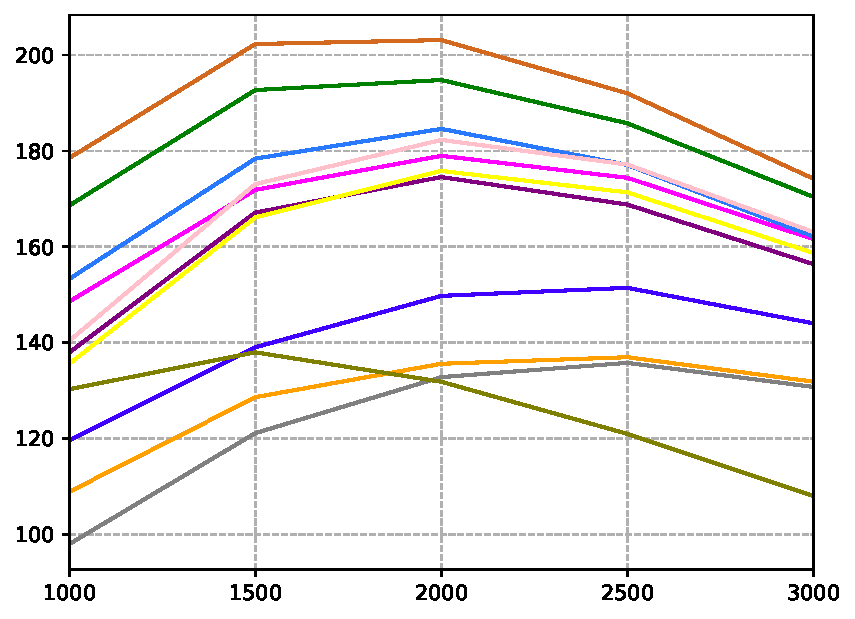
\includegraphics[width=0.24\textwidth]{figs/ft_reuters_new_auc_increase.pdf}}
		\subfloat[SQD]{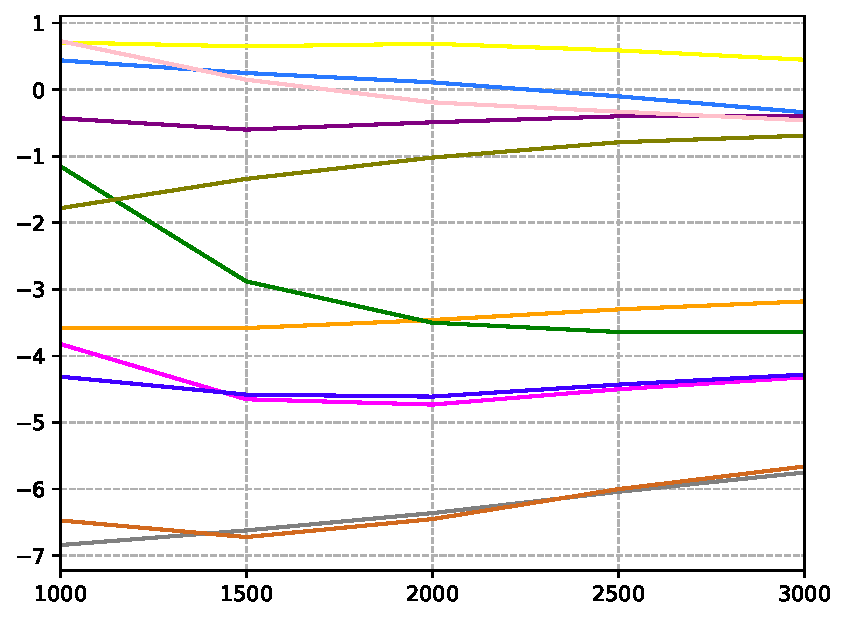
\includegraphics[width=0.24\textwidth]{figs/ft_stackoverflow_tokenized_auc_increase.pdf}}
	\end{center}
	\noindent
	\begin{center}
		\subfloat[TNEWS]{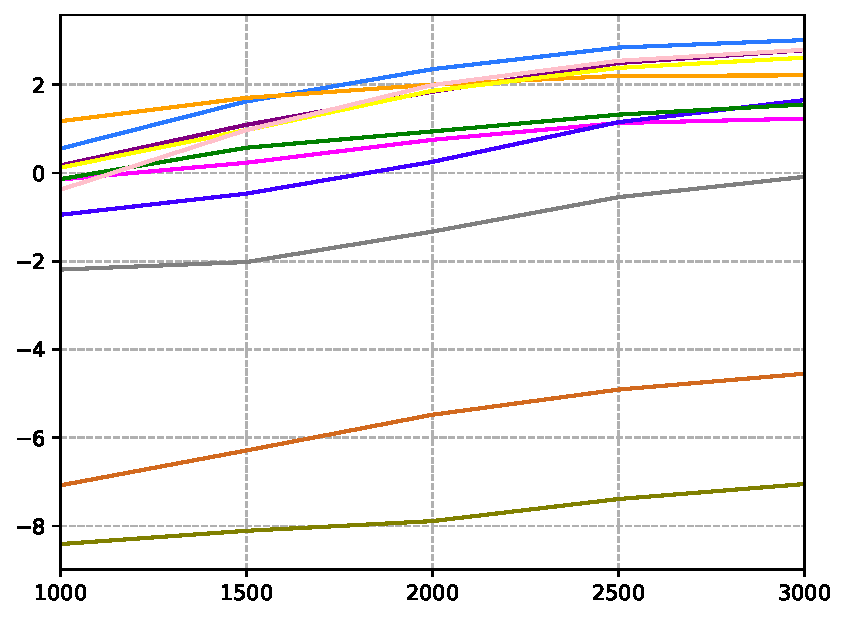
\includegraphics[width=0.24\textwidth]{figs/ft_tnews_tokenized_auc_increase.pdf}} % \newline
		\subfloat[GCS]{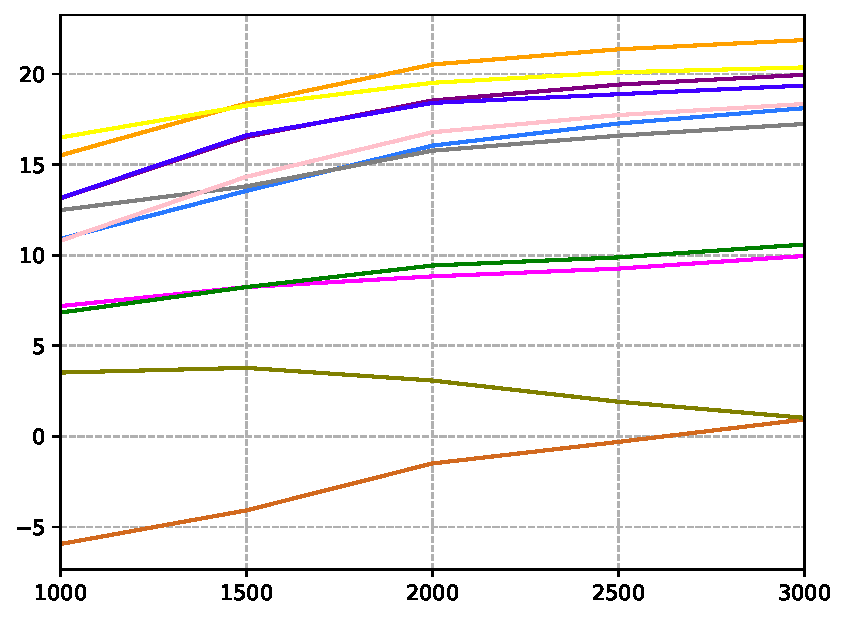
\includegraphics[width=0.24\textwidth]{figs/ft_yanjing_tokenized_auc_increase.pdf}}
	\end{center}

\noindent
\begin{center}
	\subfloat[Biomedical]{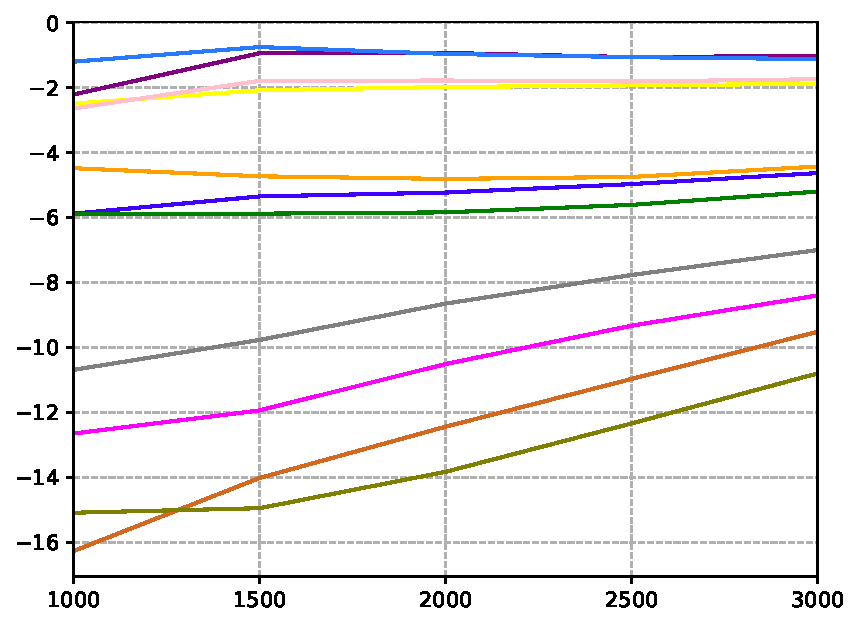
\includegraphics[width=0.24\textwidth]{figs/ft_Biomedical_tokenized_auc_increase.pdf}} % \newline
	\subfloat[StackOverflow]{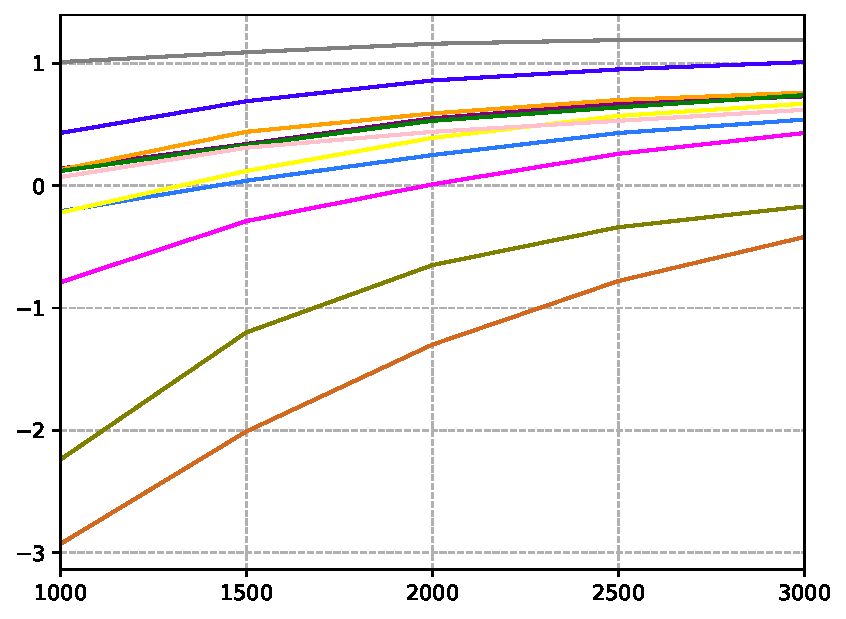
\includegraphics[width=0.24\textwidth]{figs/ft_so_tokenized_auc_increase.pdf}}
\end{center}
\noindent
\begin{center}
	\subfloat[SearchSnippets]{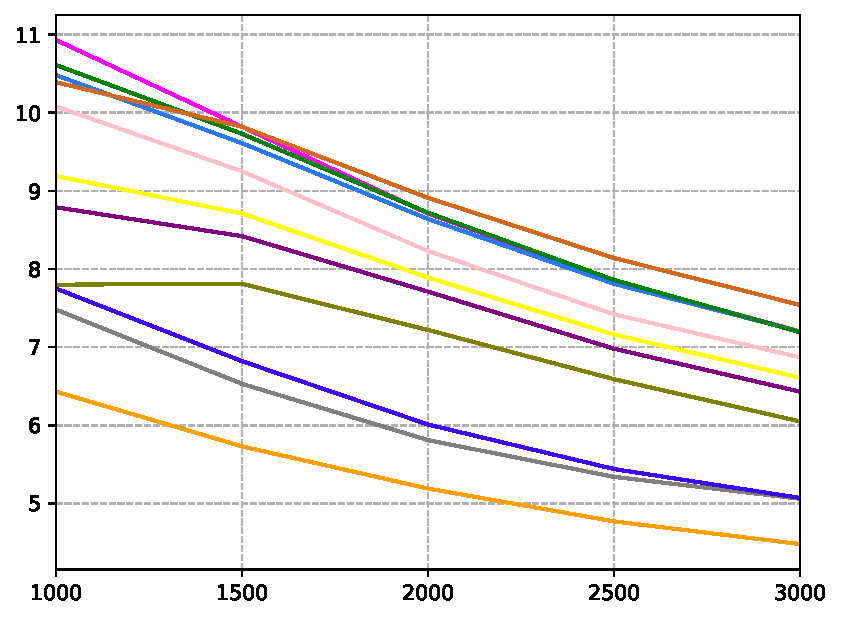
\includegraphics[width=0.24\textwidth]{figs/ft_SearchSnippets_tokenized_auc_increase.pdf}} % \newline
\end{center}
	\caption{Increase percent using FastText}
	\label{fig:auc_increase_ft}
\end{figure}

\begin{figure}[th!]%[!hbt]
	\noindent
	\begin{center}
		\subfloat[Reuters]{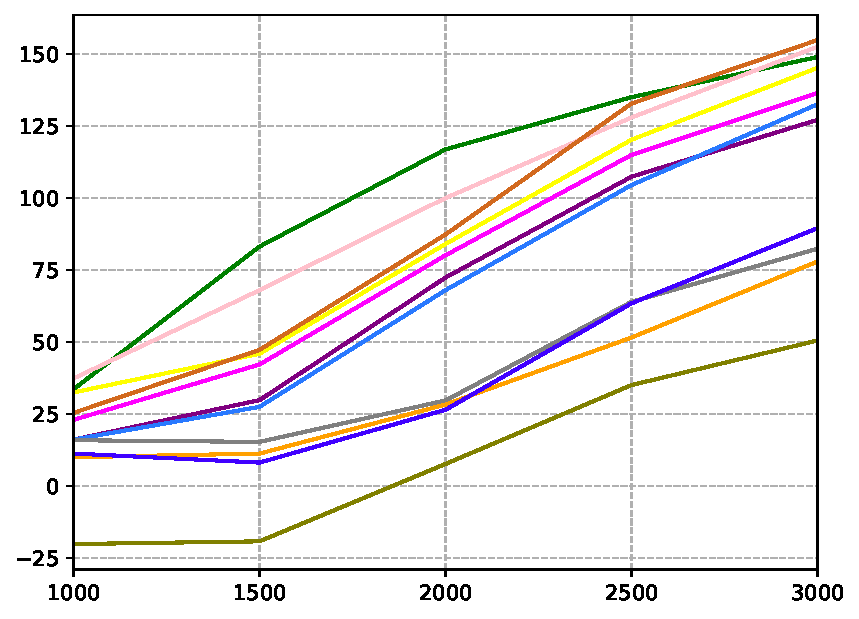
\includegraphics[width=0.24\textwidth]{figs/bert_reuters_new_auc_increase.pdf}}
		\subfloat[SQD]{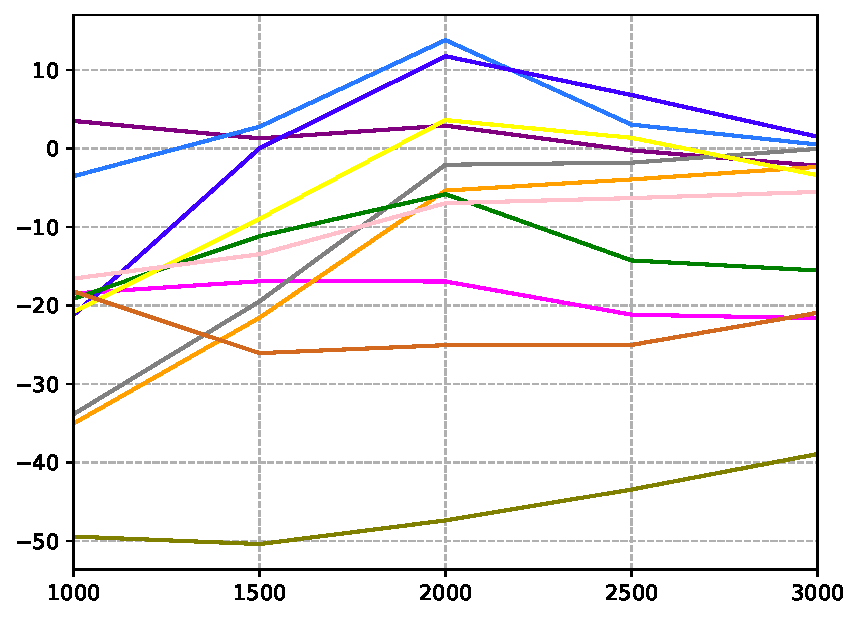
\includegraphics[width=0.24\textwidth]{figs/bert_stack_merge_auc_increase.pdf}}
	\end{center}
	\noindent
	\begin{center}
		\subfloat[TNEWS]{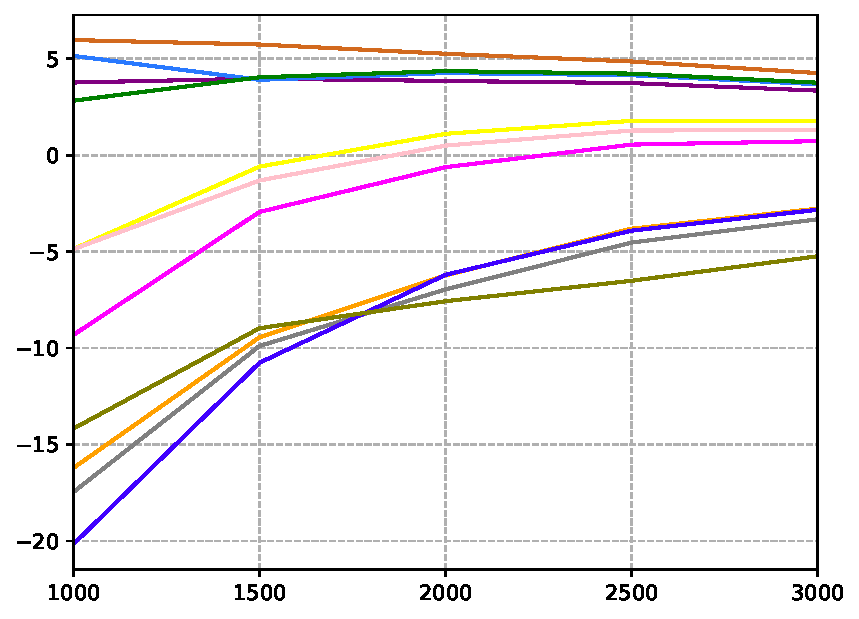
\includegraphics[width=0.24\textwidth]{figs/bert_tnews_auc_increase.pdf}} % \newline
		\subfloat[GCS]{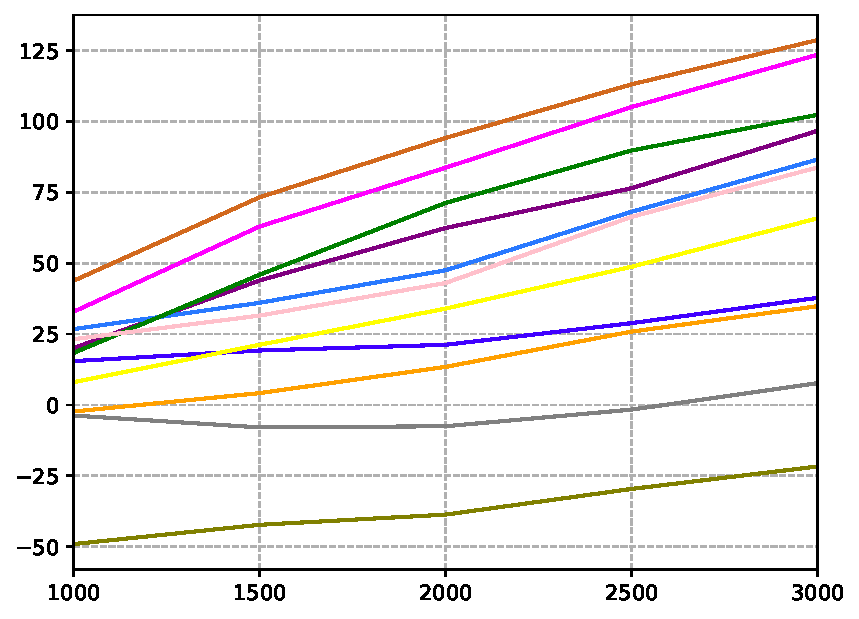
\includegraphics[width=0.24\textwidth]{figs/bert_yanjing_merge_auc_increase.pdf}}
	\end{center}
\noindent
\begin{center}
	\subfloat[Biomedical]{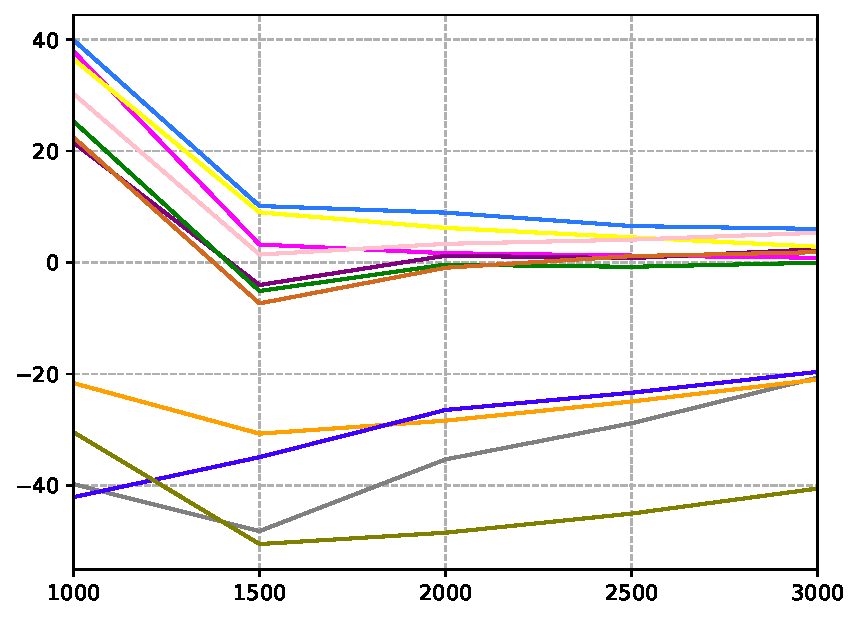
\includegraphics[width=0.24\textwidth]{figs/bert_Bio_auc_increase.pdf}} % \newline
	\subfloat[StackOverflow]{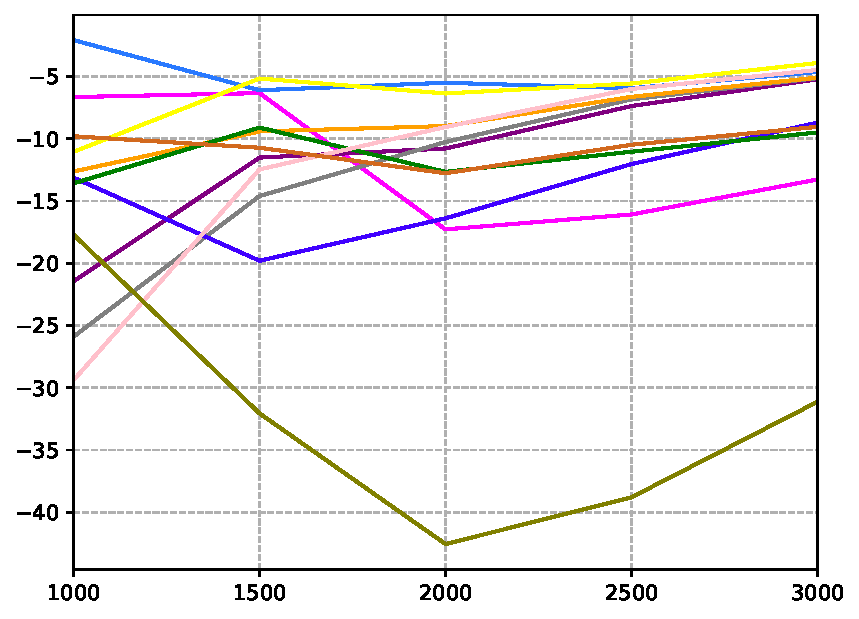
\includegraphics[width=0.24\textwidth]{figs/bert_SO_auc_increase.pdf}}
\end{center}
\noindent
\begin{center}
	\subfloat[SearchSnippets]{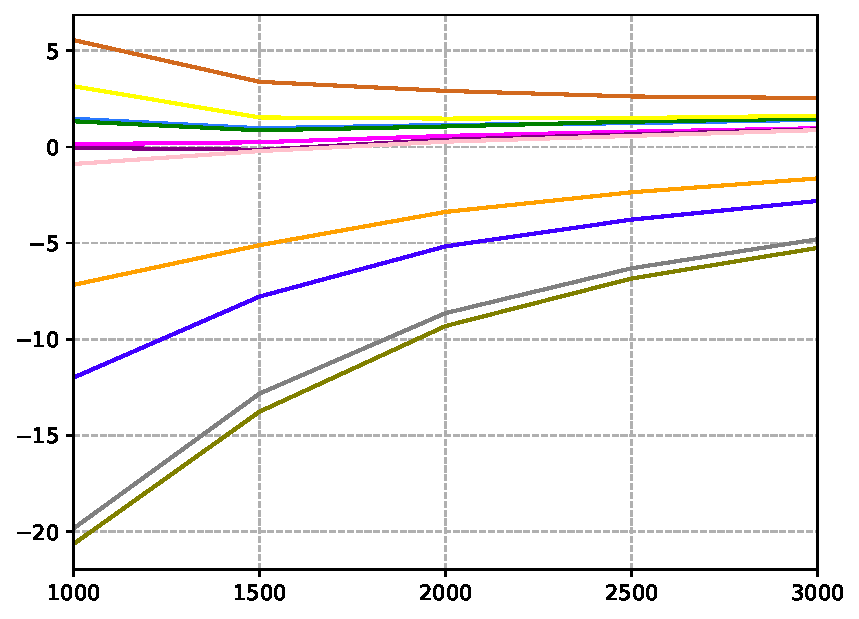
\includegraphics[width=0.24\textwidth]{figs/bert_Search_auc_increase.pdf}} % \newline
\end{center}
	\caption{Increase percent using BERT}
	\label{fig:auc_increase_bert}
\end{figure}

\begin{figure}[th!]%[!hbt]
	\noindent
	\begin{center}
		\subfloat[Reuters]{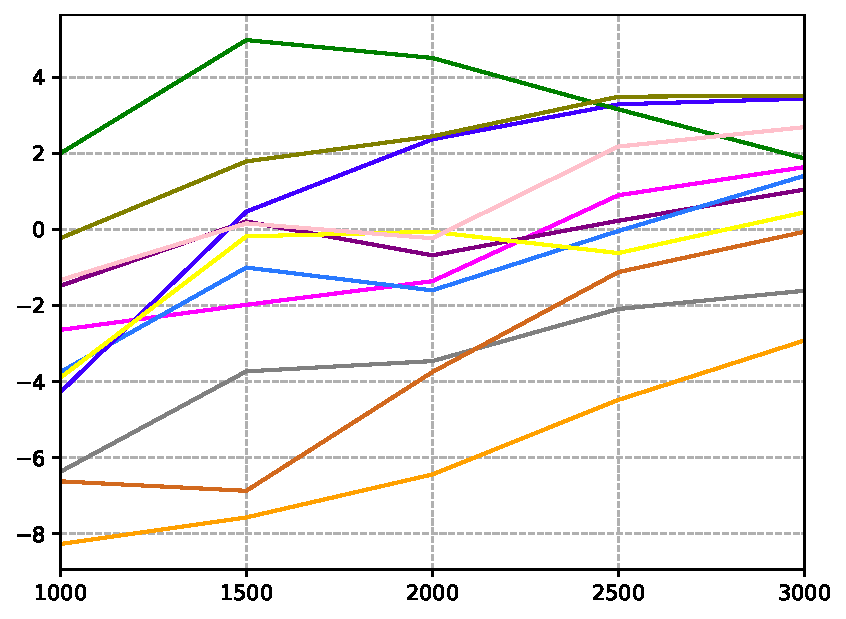
\includegraphics[width=0.24\textwidth]{figs/lstm_pytorch_reuters_new_merge_auc_increase.pdf}}
		\subfloat[SQD]{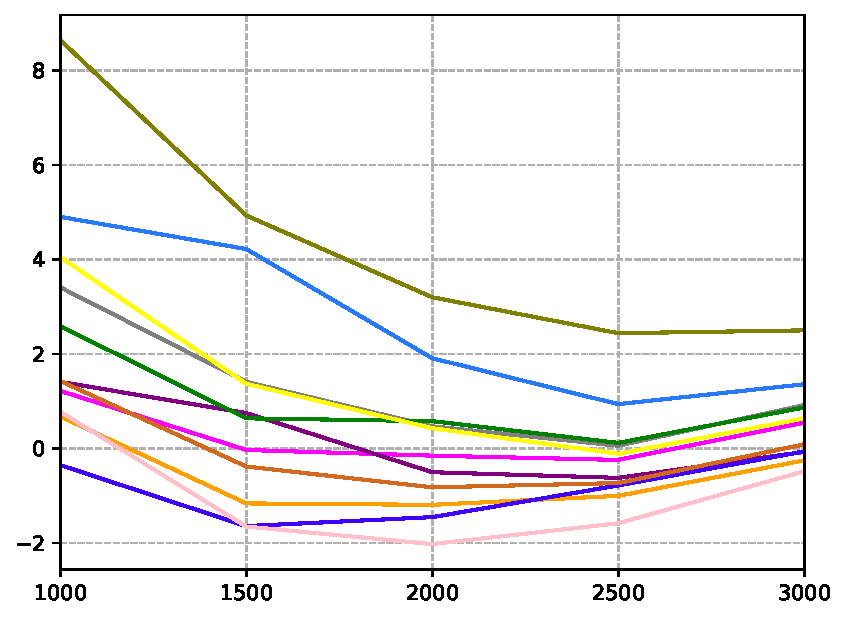
\includegraphics[width=0.24\textwidth]{figs/lstm_pytorch_stackoverflow_tokenized_merge_auc_increase.pdf}}
	\end{center}
	\noindent
	\begin{center}
		\subfloat[TNEWS]{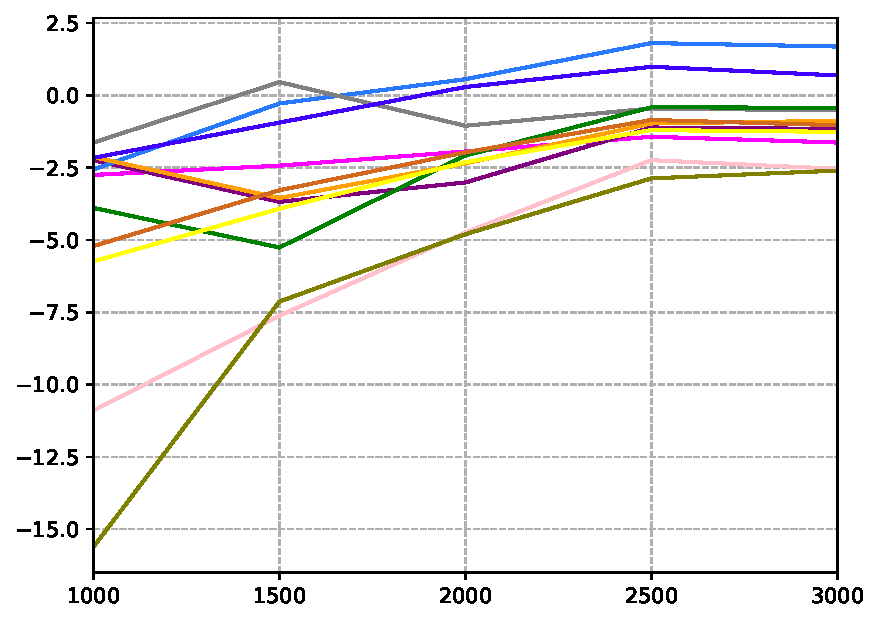
\includegraphics[width=0.24\textwidth]{figs/lstm_pytorch_tnews_tokenized_merge_auc_increase.pdf}} % \newline
		\subfloat[GCS]{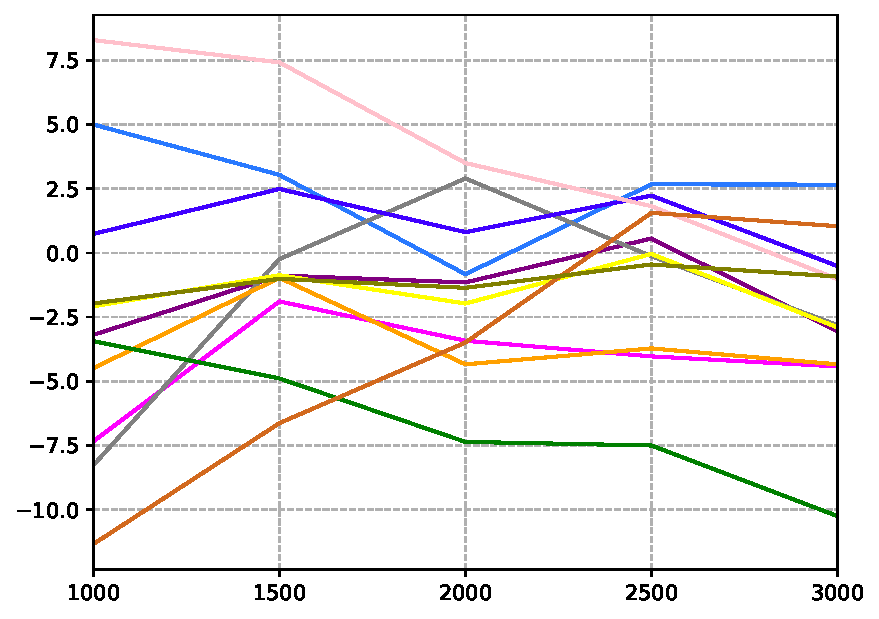
\includegraphics[width=0.24\textwidth]{figs/lstm_pytorch_yanjing_tokenized_merge_auc_increase.pdf}}
	\end{center}
	\noindent
	\begin{center}
		\subfloat[Biomedical]{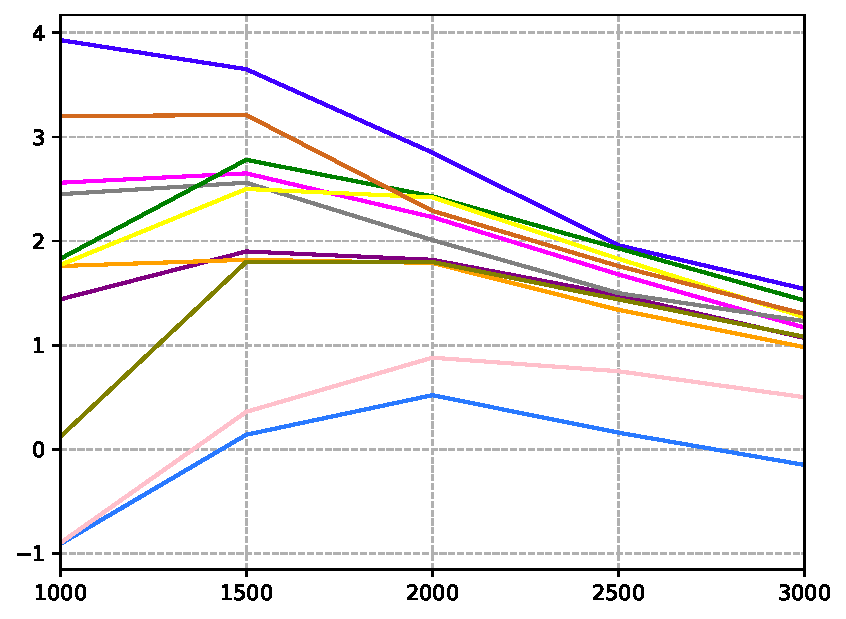
\includegraphics[width=0.24\textwidth]{figs/lstm_pytorch_Biomedical_tokenized_auc_increase.pdf}} % \newline
		\subfloat[StackOverflow]{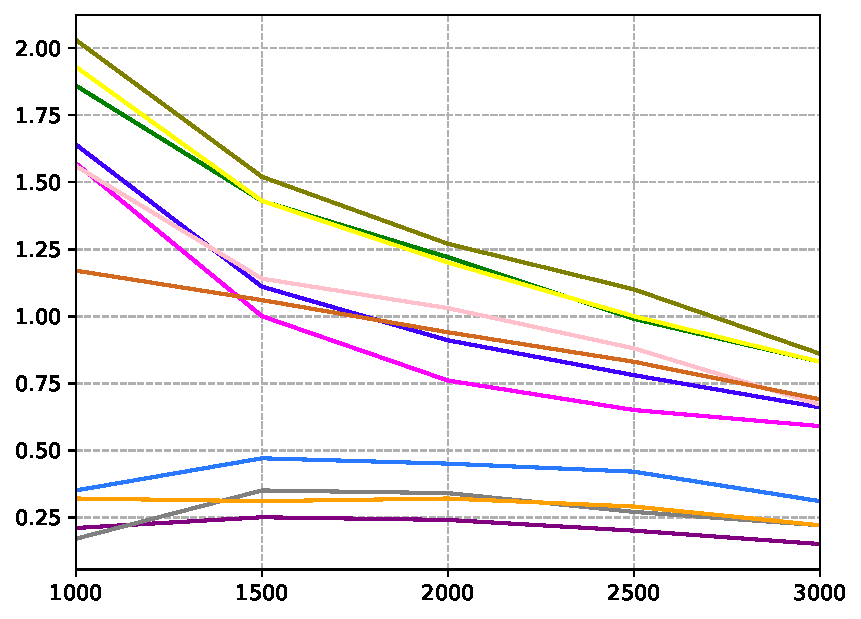
\includegraphics[width=0.24\textwidth]{figs/lstm_pytorch_StackOverflow_tokenized_auc_increase.pdf}}
	\end{center}
	\noindent
	\begin{center}
		\subfloat[SearchSnippets]{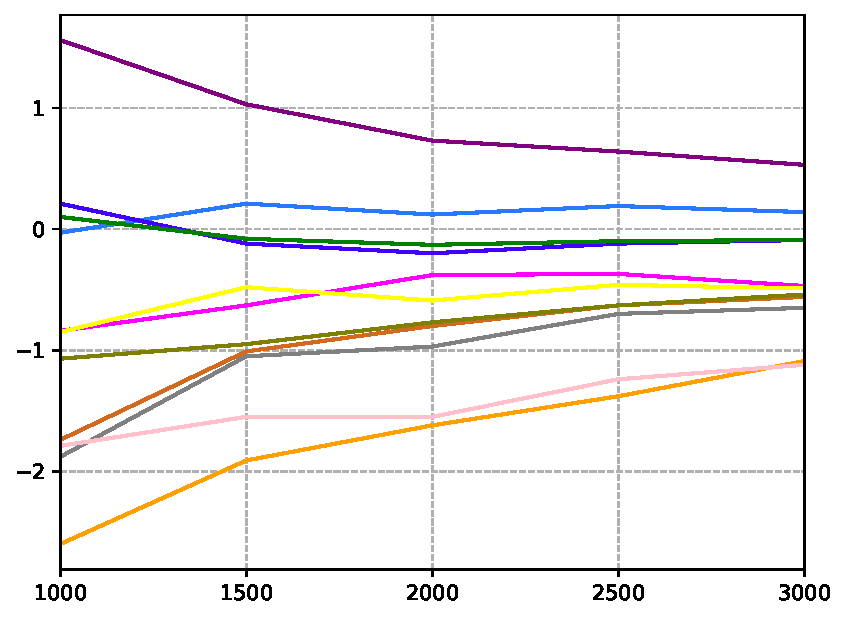
\includegraphics[width=0.24\textwidth]{figs/lstm_pytorch_SearchSnippets_tokenized_auc_increase.pdf}} % \newline
	\end{center}
	\caption{Increase percent using LSTM+ATTN}
	\label{fig:auc_increase_lstm}
\end{figure}

\begin{figure}[th!]%[!hbt]
	\noindent
	\begin{center}
		\subfloat[Reuters]{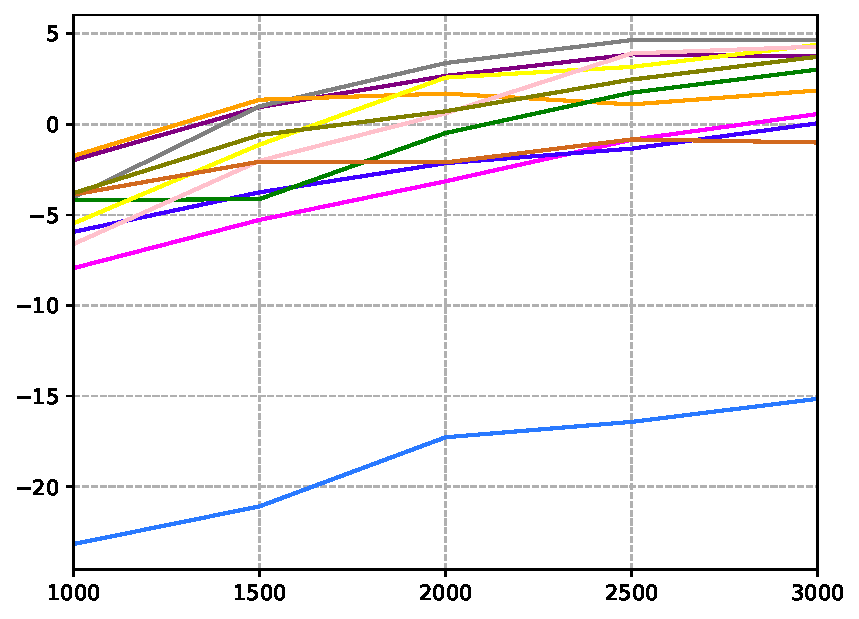
\includegraphics[width=0.24\textwidth]{figs/cnn_pytorch_reuters_new_merge_auc_increase.pdf}}
		\subfloat[SQD]{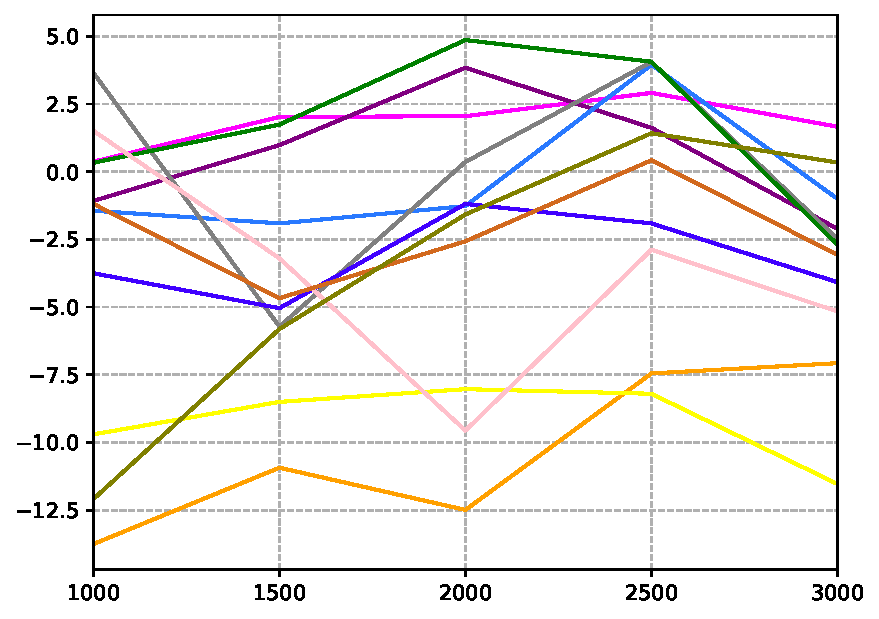
\includegraphics[width=0.24\textwidth]{figs/cnn_pytorch_stackoverflow_tokenized_merge_auc_increase.pdf}}
	\end{center}
	\noindent
	\begin{center}
		\subfloat[TNEWS]{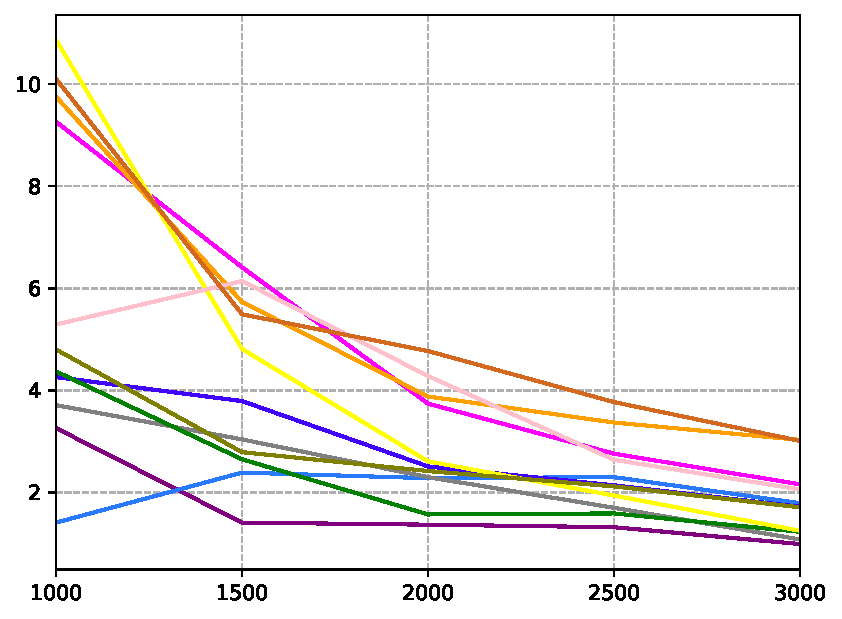
\includegraphics[width=0.24\textwidth]{figs/cnn_pytorch_tnews_tokenized_merge_auc_increase.pdf}} % \newline
		\subfloat[GCS]{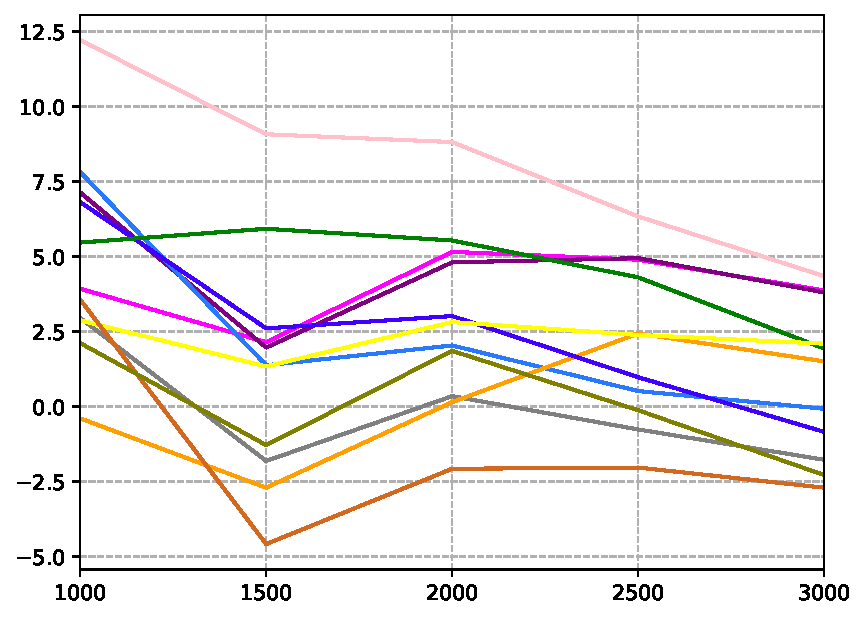
\includegraphics[width=0.24\textwidth]{figs/cnn_pytorch_yanjing_tokenized_merge_auc_increase.pdf}}
	\end{center}
	\noindent
	\begin{center}
		\subfloat[Biomedical]{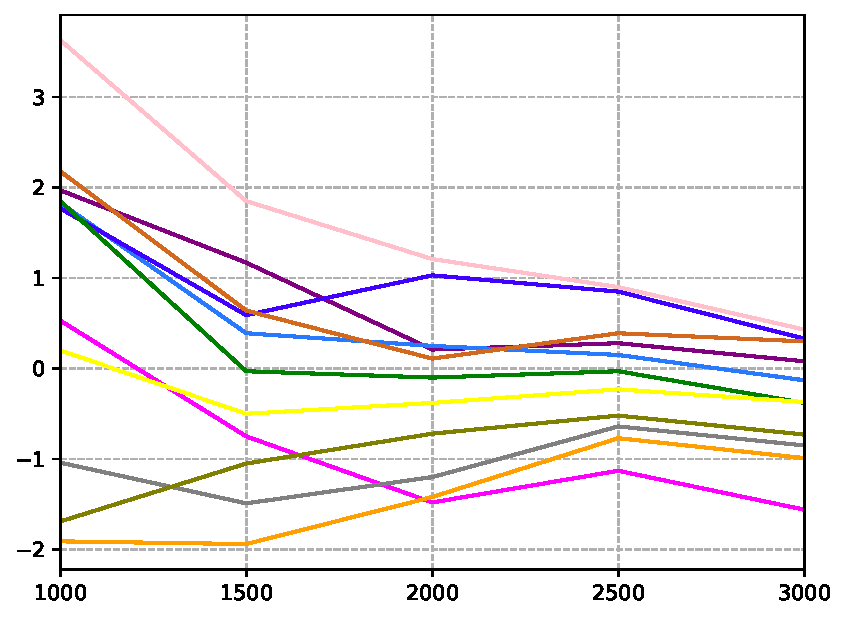
\includegraphics[width=0.24\textwidth]{figs/cnn_pytorch_Biomedical_tokenized_auc_increase.pdf}} % \newline
		\subfloat[StackOverflow]{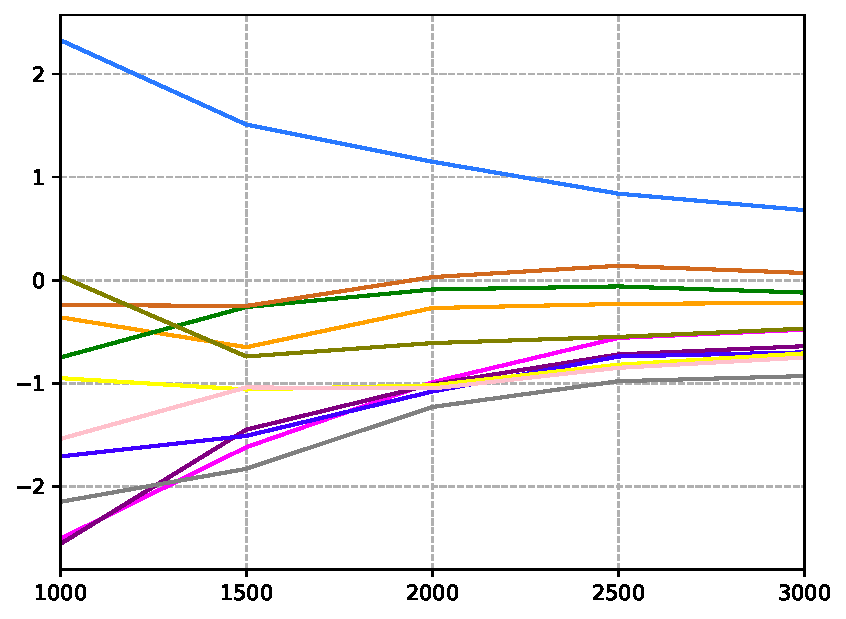
\includegraphics[width=0.24\textwidth]{figs/cnn_pytorch_SO_tokenized_auc_increase.pdf}}
	\end{center}
	\noindent
	\begin{center}
		\subfloat[SearchSnippets]{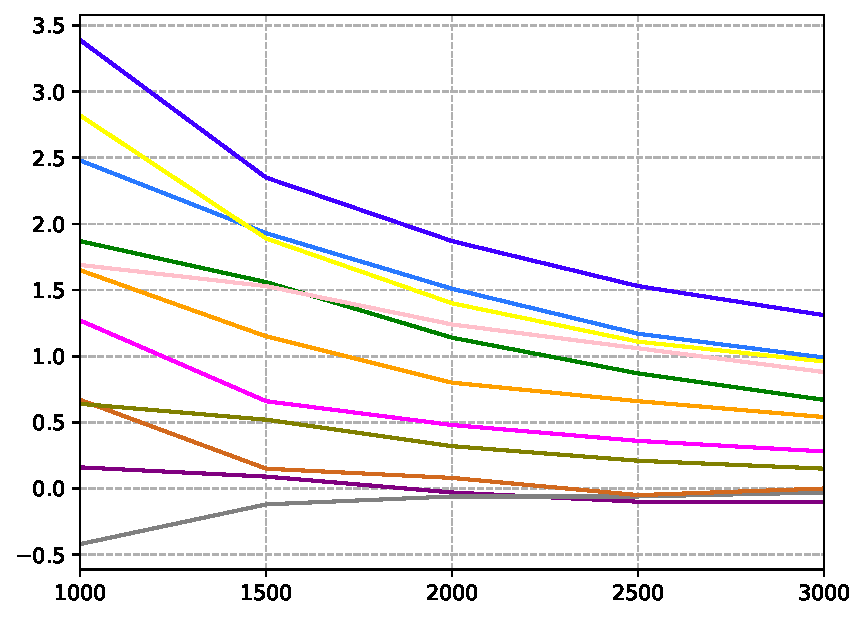
\includegraphics[width=0.24\textwidth]{figs/cnn_pytorch_SearchSnippets_tokenized_auc_increase.pdf}} % \newline
	\end{center}
	\caption{Increase percent using CNN}
	\label{fig:auc_increase_cnn}
\end{figure}

\begin{table*}[th]
	\scriptsize
	\centering
	\begin{tabular}{cccccccc}
		\toprule
		Model & Reuters    & SQD   & TNEWS   & GCS& Biomedical & StackOverflow & SearchSnippets\\ \hline
		fastText & 2.79 & 1.01 & 1.01 & 1.16 & 0.99 & 1.01 & 1.11 \\
		BERT & 1.37 & 1.03 & 1.06 & 1.44 & 1.4 & 0.98 & 1.06 \\
		LSTM+ATTN & 1.02 & 1.09 & 0.98 & 1.08 & 1.04 & 1.02 & 1.02 \\
		CNN & 0.98 & 1.04 & 1.11 & 1.12 & 1.04 & 1.02 & 1.03 \\
		
		\bottomrule
	\end{tabular}
	\caption{AUC* ratio between best method (exclude Random) and Random when \#samples=1000}
	\label{table:auc_ratio_1000}
\end{table*}

\begin{table*}[th]
	\scriptsize
	\centering
	\begin{tabular}{cccccccc}
		\toprule
		Model & Reuters    & SQD   & TNEWS   & GCS& Biomedical & StackOverflow & SearchSnippets\\ \hline
		fastText & 3.03 & 1.01 & 1.02 & 1.21 & 0.99 & 1.01 & 1.09 \\
		BERT & 2.17 & 1.14 & 1.05 & 1.94 & 1.09 & 0.94 & 1.03 \\
		LSTM+ATTN & 1.05 & 1.03 & 1.01 & 1.04 & 1.03 & 1.01 & 1.01 \\
		CNN & 1.03 & 1.05 & 1.05 & 1.09 & 1.01 & 1.01 & 1.02 \\
		
		\bottomrule
	\end{tabular}
	\caption{AUC* ratio between best method (exclude Random) and Random when \#samples=2000}
	\label{table:auc_ratio_2000}
\end{table*}

\begin{table*}[th]
	\scriptsize
	\centering
	\begin{tabular}{cccccccc}
		\toprule
		Model & Reuters    & SQD   & TNEWS   & GCS& Biomedical & StackOverflow & SearchSnippets\\ \hline
		fastText & 2.74 & 1.0 & 1.03 & 1.22 & 0.99 & 1.01 & 1.08 \\
		BERT & 2.55 & 1.01 & 1.04 & 2.29 & 1.06 & 0.96 & 1.03 \\
		LSTM+ATTN & 1.04 & 1.02 & 1.02 & 1.03 & 1.02 & 1.01 & 1.01 \\
		CNN & 1.05 & 1.02 & 1.03 & 1.04 & 1.0 & 1.01 & 1.01 \\
		
		\bottomrule
	\end{tabular}
	\caption{AUC* ratio between best method (exclude Random) and Random when \#samples=3000}
	\label{table:auc_ratio}
\end{table*}

\begin{table*}[th]
	\scriptsize
	\centering
	\begin{tabular}{cccccccc}
		\toprule
		Model & Reuters    & SQD   & TNEWS   & GCS& Biomedical & StackOverflow & SearchSnippets\\ \hline
		fastText & 0.37 & 0.8 & 0.82 & 0.67 & 0.7 & 0.9 & 0.93\\
		BERT & 0.34 & 0.83 & 0.82 & 0.63 & 0.7 & 0.89 & 0.95\\
		LSTM+ATTN & 0.44 & 0.82 & 0.78 & 0.53 & 0.69 & 0.89 & 0.94\\
		CNN & 0.36 & 0.41 & 0.73 & 0.39 & 0.67 & 0.86 & 0.93\\
		\bottomrule
	\end{tabular}
	\caption{Upperbound Macro F1 score (using all training samples) of different models.}
	\label{table:upperbound}
\end{table*}

Upperbound Macro F1 score (\#samples=1000,2000,3000) of different models.
AUC* ratio between best method (exclude Random) and Random when \#samples=1000
AUC* ratio between best method (exclude Random) and Random when \#samples=2000
AUC* ratio between best method (exclude Random) and Random when \#samples=3000


\begin{table*}[th]
	\scriptsize
	\centering
	\begin{tabular}{ccc}
		\toprule
		Model & Pearson's correlation coefficient & p-value\\ \hline
		fastText & -0.88 & 0.0087\\
		BERT & -0.88 & 0.0083\\
		LSTM+ATTN & -0.97 & 0.0004\\
		CNN & -0.70 & 0.0793\\
		\bottomrule
	\end{tabular}
	\caption{Pearson correlation coefficient
		 between AUC* ratio and Upperbound Macro F1 score of different models.}
	\label{table:pearson}
\end{table*}



\subsubsection{Number of Samples}
Another metric provided in the proposal is the query number of designed methods should be 50\% less than the baseline system when the precision and recall rate of every label class achieves 85\% as well as 50\% respectively. The decrease rate is calculated as follows.

$$decrease\ percent = \frac{N_{Random}^{i}-N_{method}^{j}}{N_{Random}} \times 100\%,$$
where $j = argmin_{k} |F1_{Random}^{i} - F1_{method}^{k}|$. $N_{Random}^{i}$ is the number of samples at $i^{th}$ step using Random method and $F1_{Random}^{i}$ is macro F1 score at $i^{th}$ step using Random method.  We select macro F1 score at \#samples=1000,1500,2000,2500,3000 using Random method as \textbf{standard}.

\figref{fig:sample_decrease_ft}, \figref{fig:sample_decrease_bert} , \figref{fig:sample_decrease_lstm}, \figref{fig:sample_decrease_cnn}show the decrease percent.


\begin{figure}[th!]%[!hbt]
	\noindent
	\begin{center}
		\subfloat[Reuters]{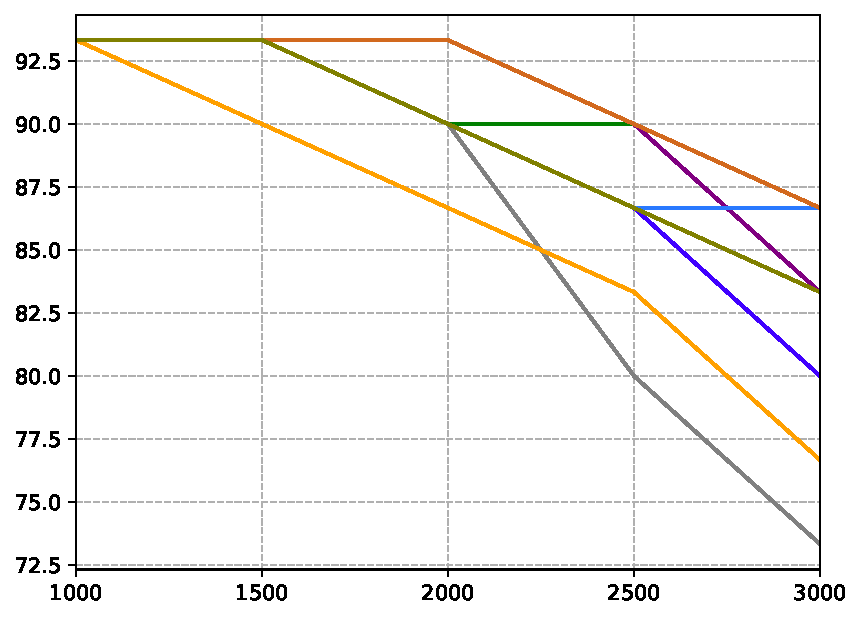
\includegraphics[width=0.24\textwidth]{figs/ft_reuters_new_sample_decrease.pdf}}
		\subfloat[SQD]{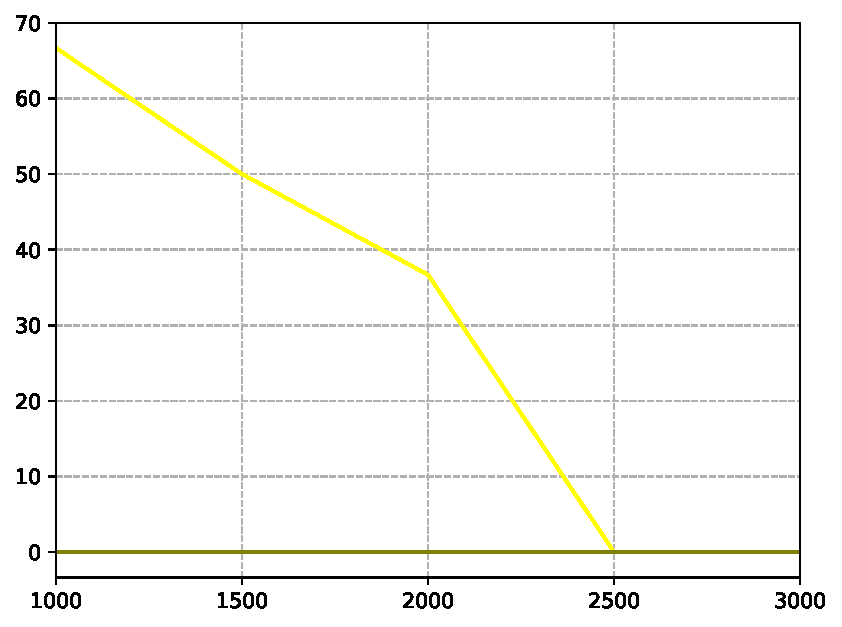
\includegraphics[width=0.24\textwidth]{figs/ft_stackoverflow_tokenized_sample_decrease.pdf}}
	\end{center}
	\noindent
	\begin{center}
		\subfloat[TNEWS]{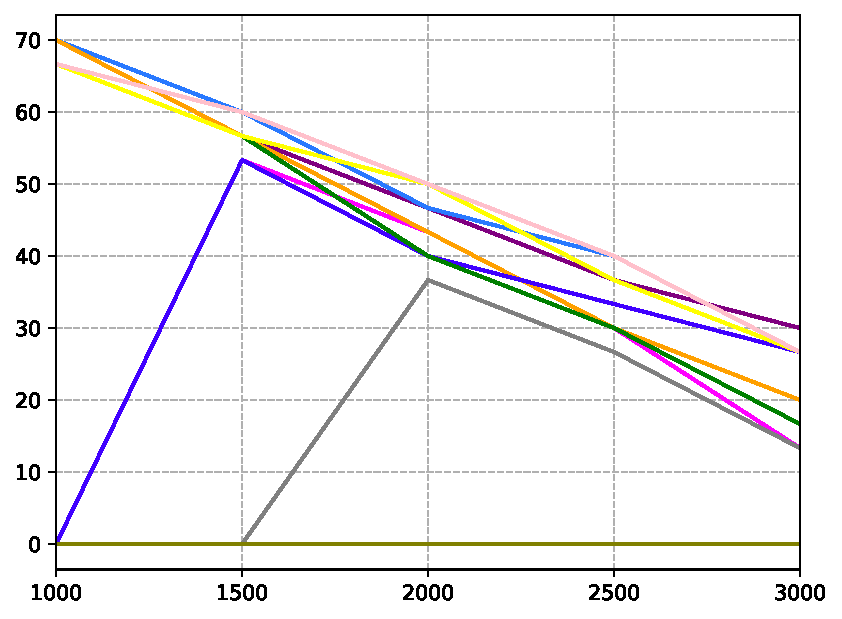
\includegraphics[width=0.24\textwidth]{figs/ft_tnews_tokenized_sample_decrease.pdf}} % \newline
		\subfloat[GCS]{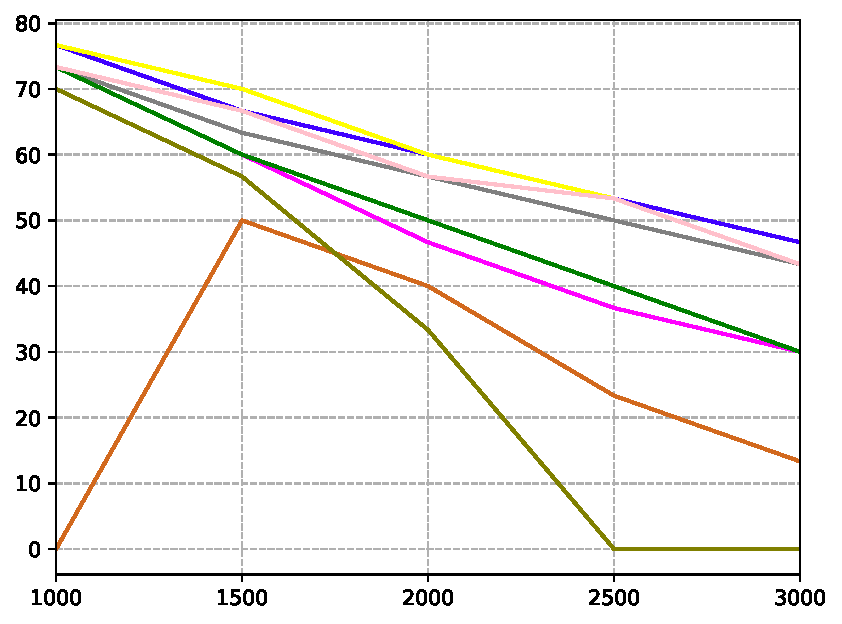
\includegraphics[width=0.24\textwidth]{figs/ft_yanjing_tokenized_sample_decrease.pdf}}
	\end{center}
\noindent
\begin{center}
	\subfloat[Biomedical]{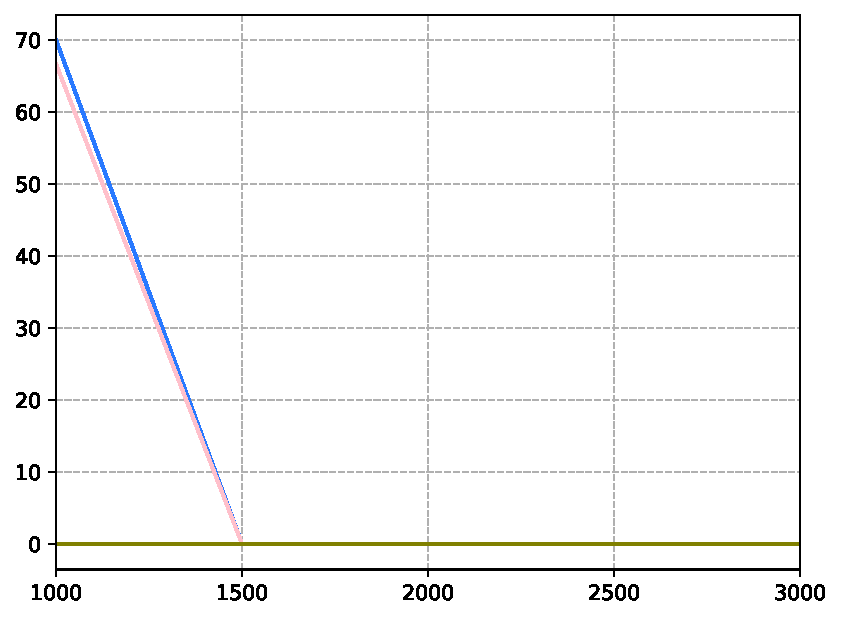
\includegraphics[width=0.24\textwidth]{figs/ft_Biomedical_tokenized_sample_decrease.pdf}} % \newline
	\subfloat[StackOverflow]{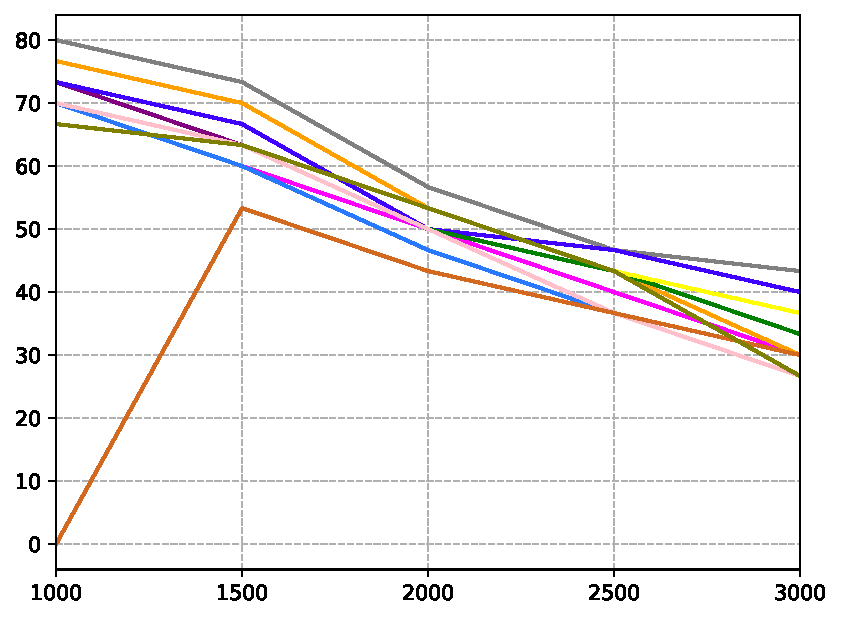
\includegraphics[width=0.24\textwidth]{figs/ft_SO_tokenized_sample_decrease.pdf}}
\end{center}
\noindent
\begin{center}
	\subfloat[SearchSnippets]{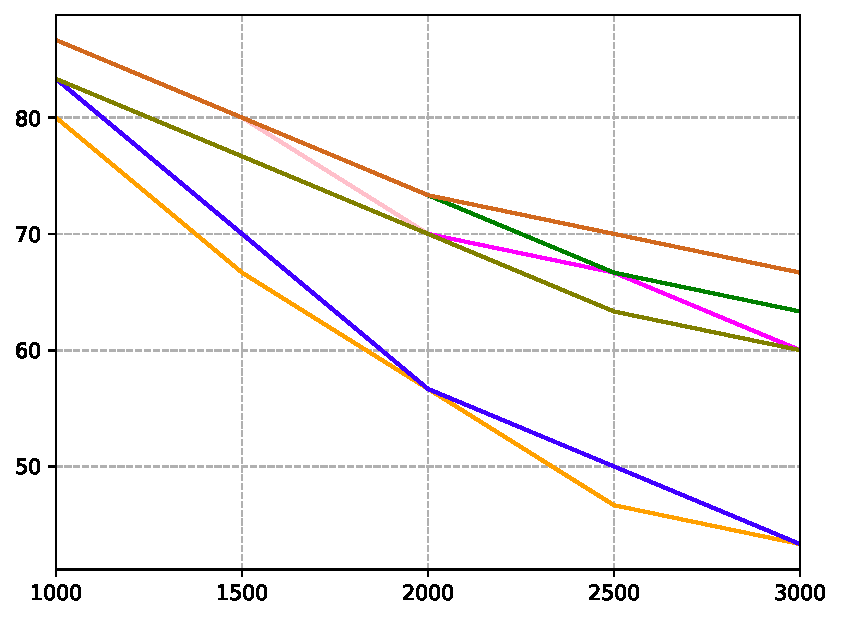
\includegraphics[width=0.24\textwidth]{figs/ft_SearchSnippets_tokenized_sample_decrease.pdf}} % \newline
\end{center}
	\caption{Decrease percent using fastText}
	\label{fig:sample_decrease_ft}
\end{figure}

\begin{figure}[th!]%[!hbt]
	\noindent
	\begin{center}
		\subfloat[Reuters]{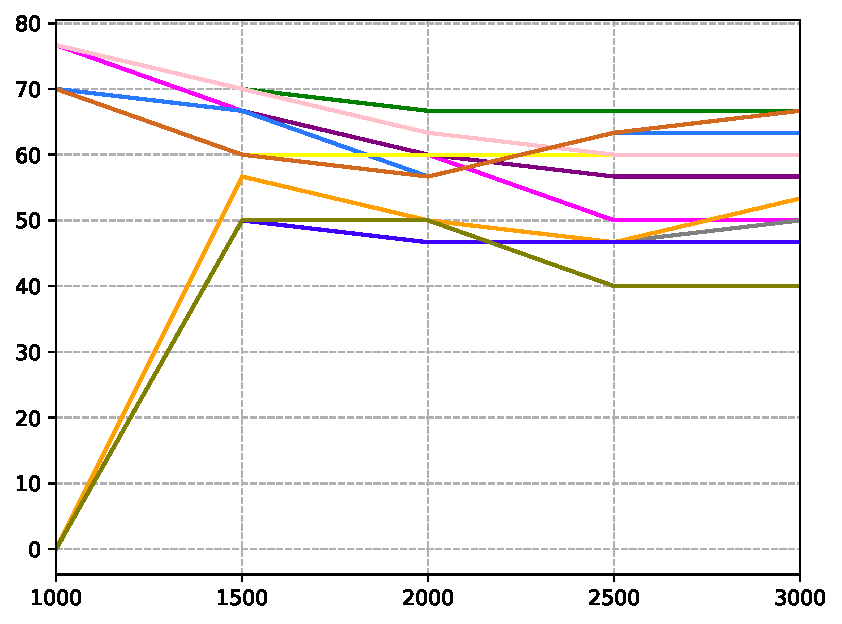
\includegraphics[width=0.24\textwidth]{figs/bert_reuters_new_sample_decrease.pdf}}
		\subfloat[SQD]{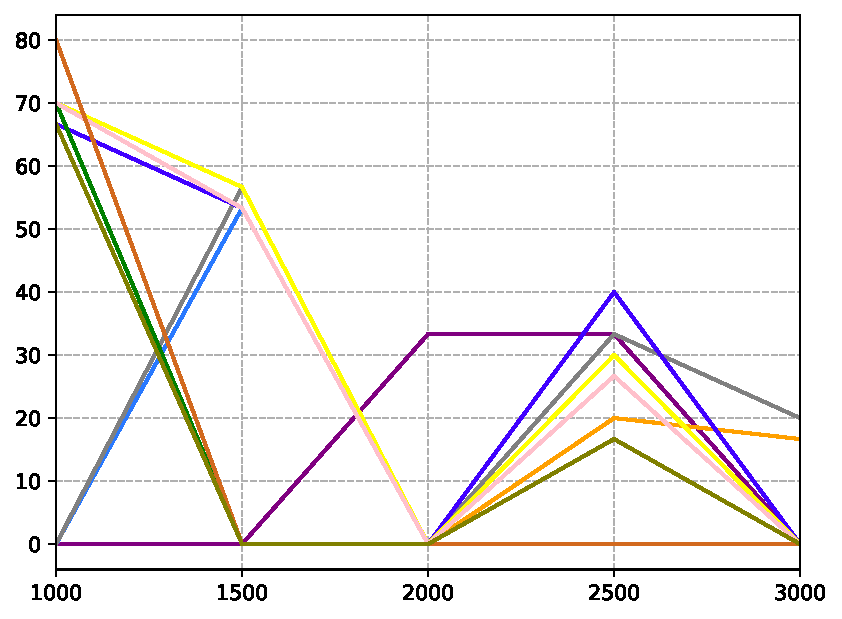
\includegraphics[width=0.24\textwidth]{figs/bert_stack_merge_sample_decrease.pdf}}
	\end{center}
	\noindent
	\begin{center}
		\subfloat[TNEWS]{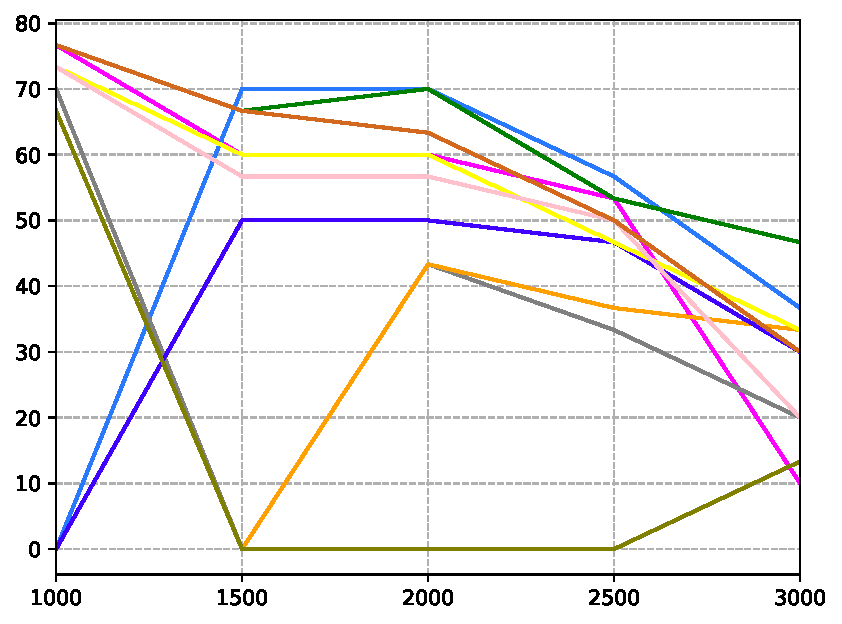
\includegraphics[width=0.24\textwidth]{figs/bert_tnews_sample_decrease.pdf}} % \newline
		\subfloat[GCS]{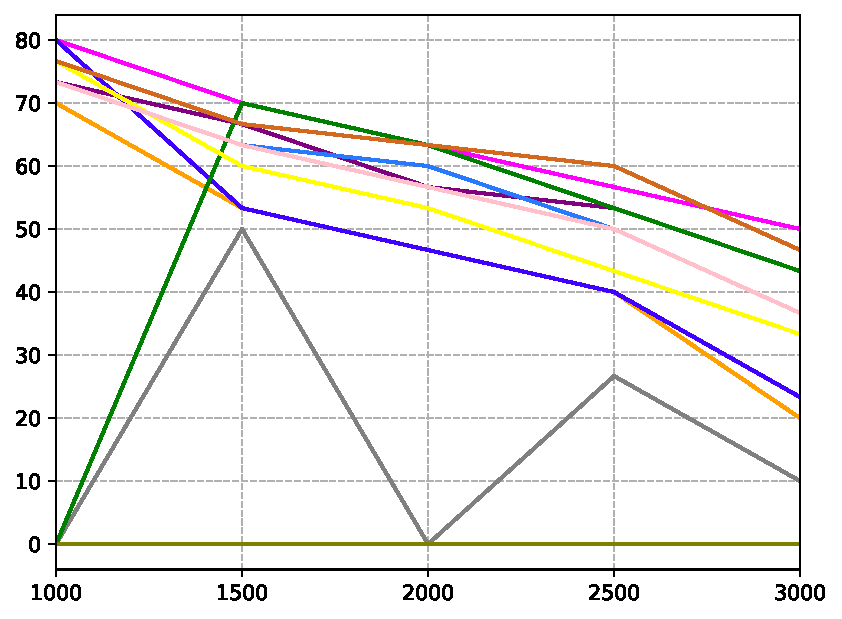
\includegraphics[width=0.24\textwidth]{figs/bert_yanjing_merge_sample_decrease.pdf}}
	\end{center}
\noindent
\begin{center}
	\subfloat[Biomedical]{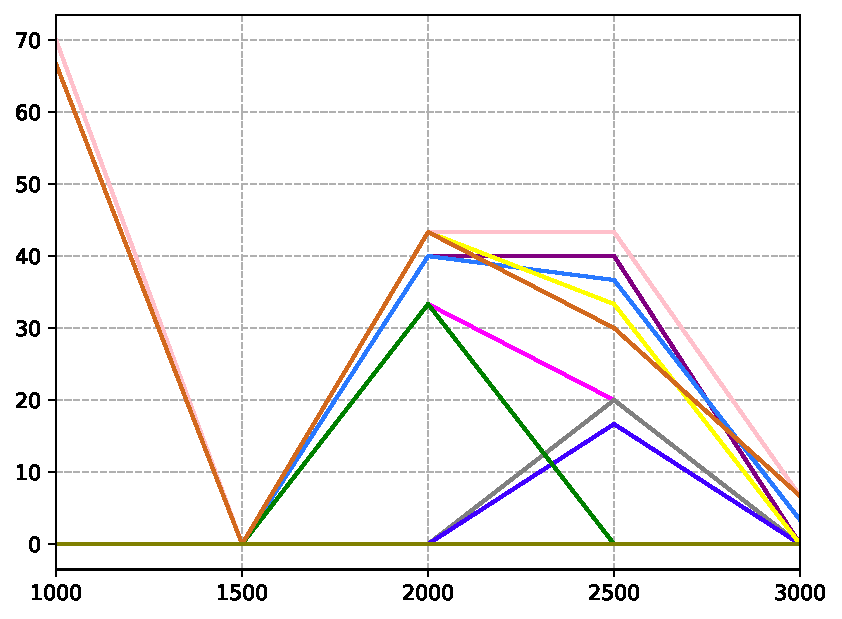
\includegraphics[width=0.24\textwidth]{figs/bert_Bio_sample_decrease.pdf}} % \newline
	\subfloat[StackOverflow]{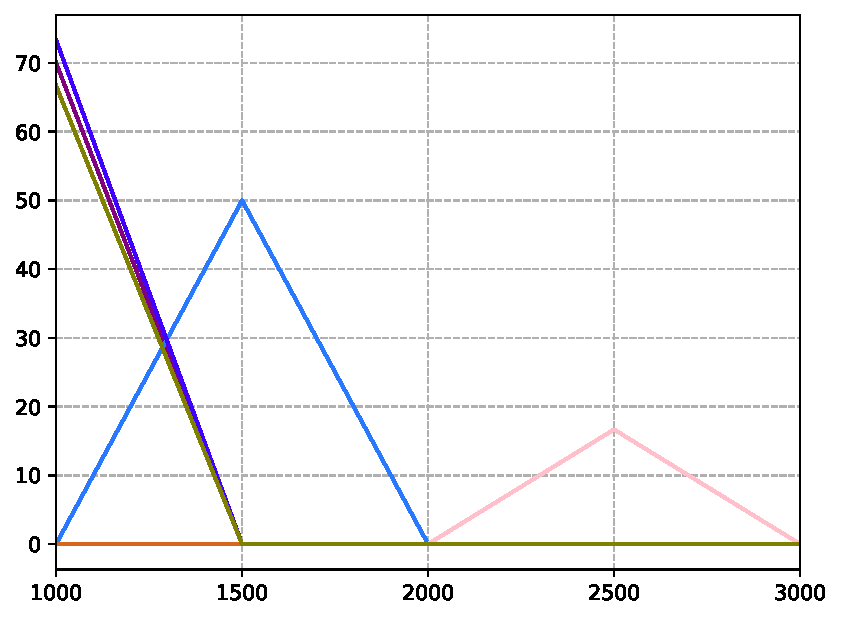
\includegraphics[width=0.24\textwidth]{figs/bert_SO_sample_decrease.pdf}}
\end{center}
\noindent
\begin{center}
	\subfloat[SearchSnippets]{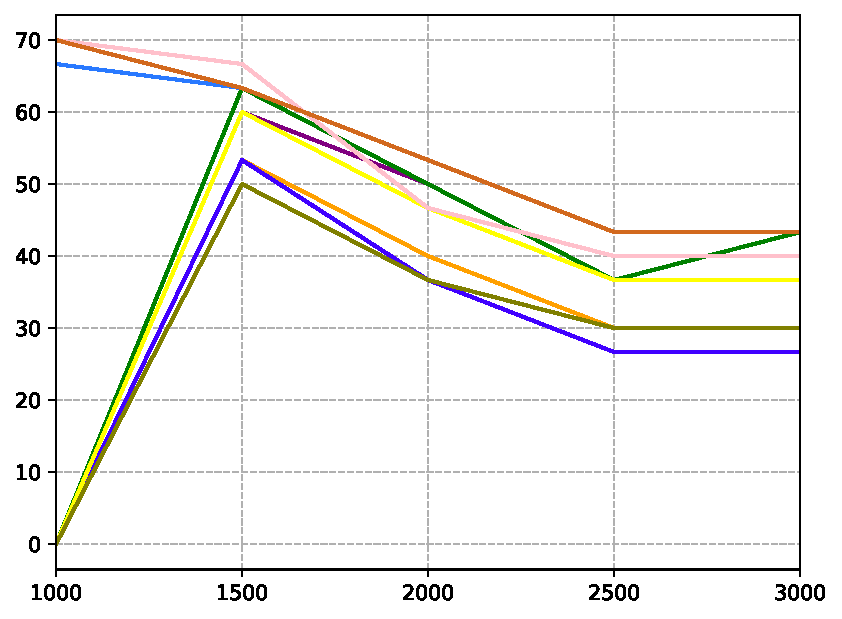
\includegraphics[width=0.24\textwidth]{figs/bert_Search_sample_decrease.pdf}} % \newline
\end{center}
	\caption{Decrease percent using BERT}
	\label{fig:sample_decrease_bert}
\end{figure}

\begin{figure}[th!]%[!hbt]
	\noindent
	\begin{center}
		\subfloat[Reuters]{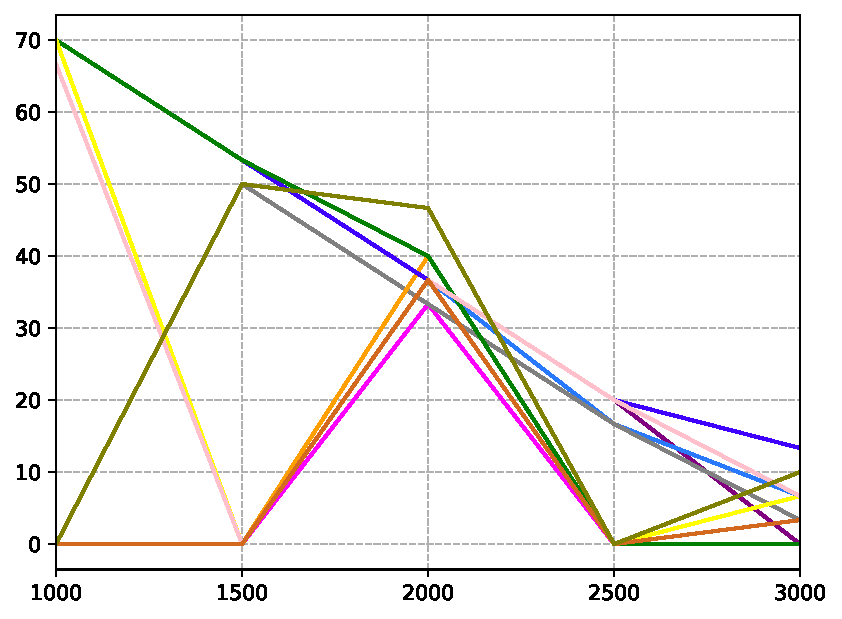
\includegraphics[width=0.24\textwidth]{figs/lstm_pytorch_reuters_new_merge_sample_decrease.pdf}}
		\subfloat[SQD]{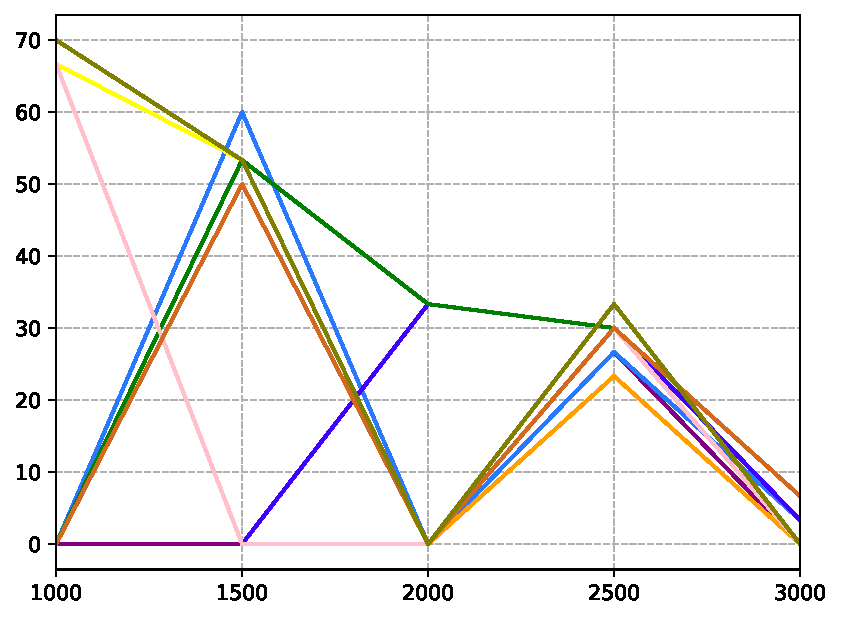
\includegraphics[width=0.24\textwidth]{figs/lstm_pytorch_stackoverflow_tokenized_merge_sample_decrease.pdf}}
	\end{center}
	\noindent
	\begin{center}
		\subfloat[TNEWS]{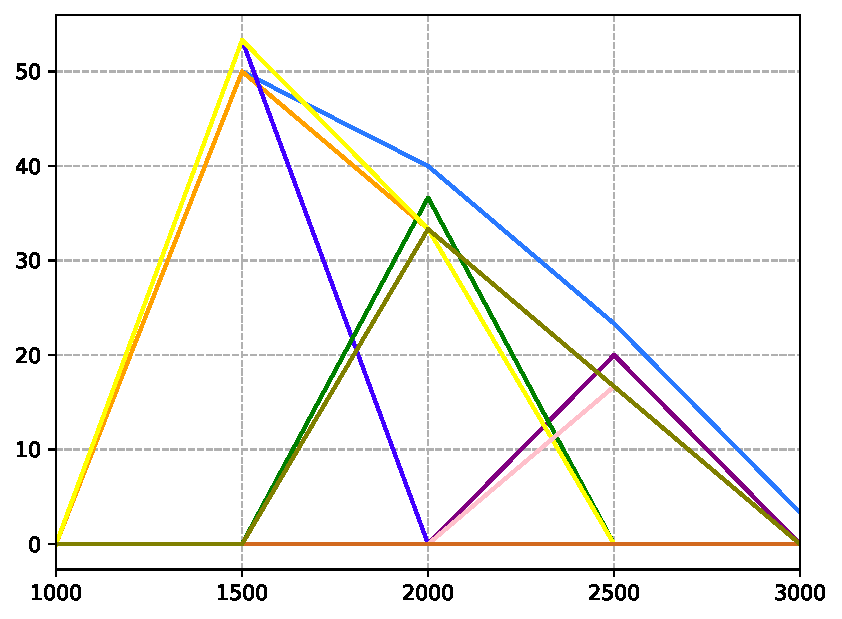
\includegraphics[width=0.24\textwidth]{figs/lstm_pytorch_tnews_tokenized_merge_sample_decrease.pdf}} % \newline
		\subfloat[GCS]{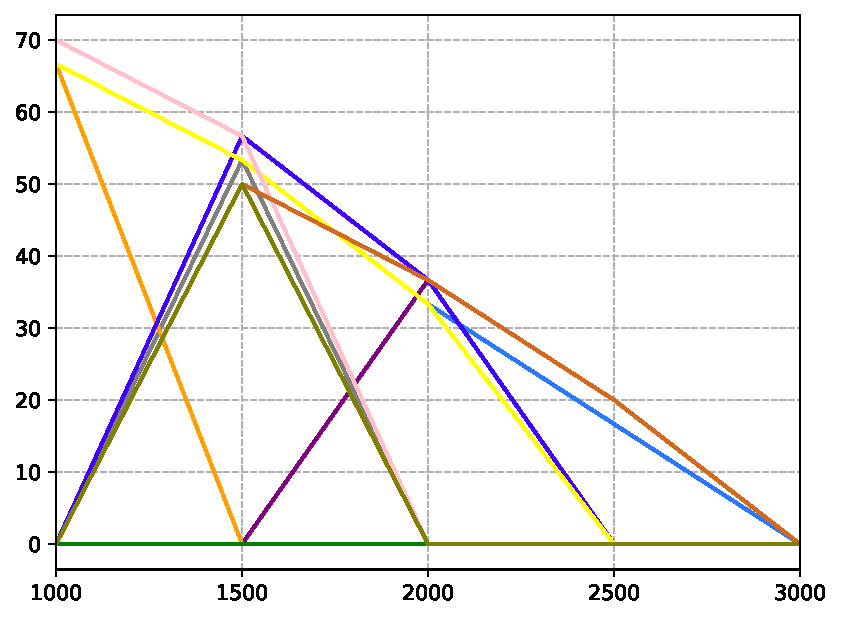
\includegraphics[width=0.24\textwidth]{figs/lstm_pytorch_yanjing_tokenized_merge_sample_decrease.pdf}}
	\end{center}
\noindent
\begin{center}
	\subfloat[Biomedical]{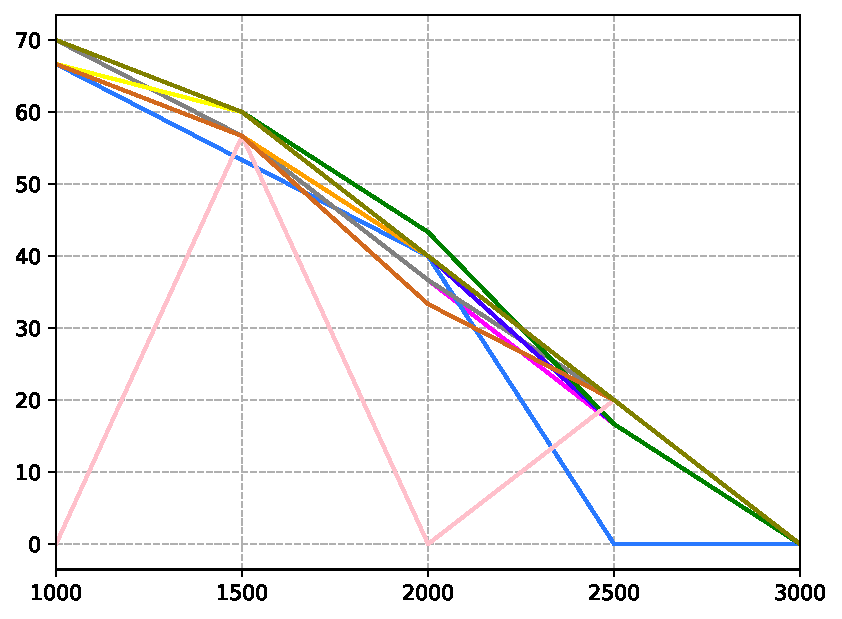
\includegraphics[width=0.24\textwidth]{figs/lstm_pytorch_Biomedical_tokenized_sample_decrease.pdf}} % \newline
	\subfloat[StackOverflow]{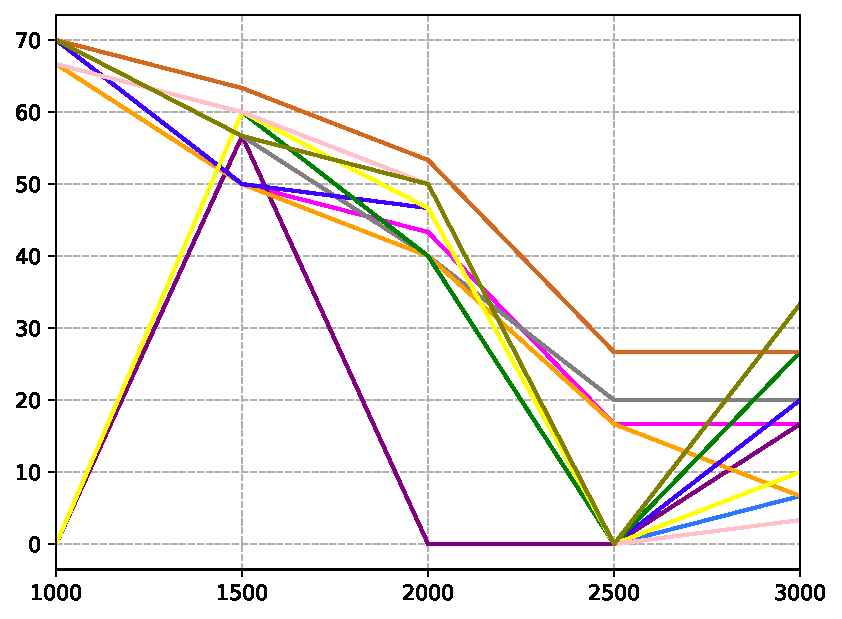
\includegraphics[width=0.24\textwidth]{figs/lstm_pytorch_SO_tokenized_sample_decrease.pdf}}
\end{center}
\noindent
\begin{center}
	\subfloat[SearchSnippets]{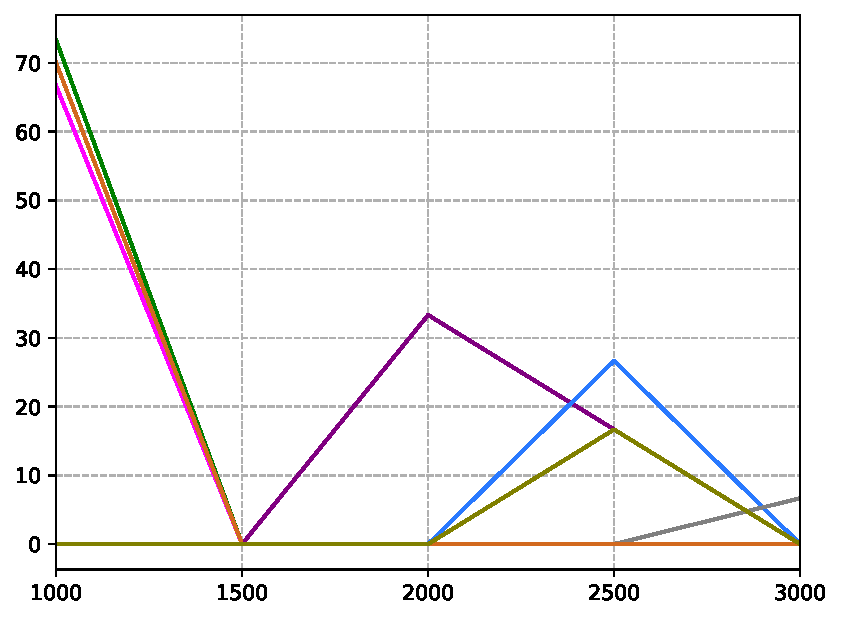
\includegraphics[width=0.24\textwidth]{figs/lstm_pytorch_SearchSnippets_tokenized_sample_decrease.pdf}} % \newline
\end{center}
	\caption{Decrease percent using LSTM+ATTN}
	\label{fig:sample_decrease_lstm}
\end{figure}

\begin{figure}[th!]%[!hbt]
	\noindent
	\begin{center}
		\subfloat[Reuters]{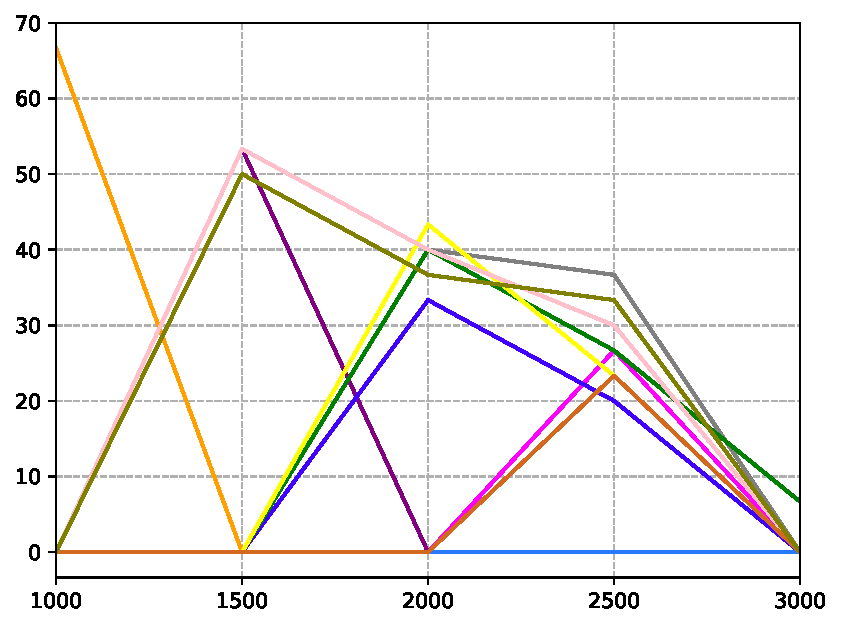
\includegraphics[width=0.24\textwidth]{figs/cnn_pytorch_reuters_new_merge_sample_decrease.pdf}}
		\subfloat[SQD]{\includegraphics[width=0.24\textwidth]{figs/cnn_pytorch_stackoverflow_tokenized_merge_sample_decrease.pdf}}
	\end{center}
	\noindent
	\begin{center}
		\subfloat[TNEWS]{\includegraphics[width=0.24\textwidth]{figs/cnn_pytorch_tnews_tokenized_merge_sample_decrease.pdf}} % \newline
		\subfloat[GCS]{\includegraphics[width=0.24\textwidth]{figs/cnn_pytorch_yanjing_tokenized_merge_sample_decrease.pdf}}
	\end{center}
	\noindent
	\begin{center}
		\subfloat[Biomedical]{\includegraphics[width=0.24\textwidth]{figs/cnn_pytorch_Biomedical_tokenized_sample_decrease.pdf}} % \newline
		\subfloat[StackOverflow]{\includegraphics[width=0.24\textwidth]{figs/cnn_pytorch_SO_tokenized_sample_decrease.pdf}}
	\end{center}
	\noindent
	\begin{center}
		\subfloat[SearchSnippets]{\includegraphics[width=0.24\textwidth]{figs/cnn_pytorch_SearchSnippets_tokenized_sample_decrease.pdf}} % \newline
	\end{center}
	\caption{Decrease percent using CNN}
	\label{fig:sample_decrease_cnn}
\end{figure}


\subsubsection{Performance on the Leyan Validation Set}
The performance of our proposed methods on the validation set should be better than or equal to the baseline system. Since only GCS provided by Leyan has figured out the validation split. We only compare the performance on GCS dataset.
\figref{fig:dev} shows Macro F1 score on GCS validation set using 4 models respectively.


\begin{figure}[th!]%[!hbt]
	\noindent
	\begin{center}
		
		\subfloat[FastText]{\includegraphics[width=0.25\textwidth, height=0.125\textheight]{figs/ft_yanjing_tokenized_dev.pdf}}
		\subfloat[BERT]{\includegraphics[width=0.25\textwidth, height=0.125\textheight]{figs/bert_yanjing_merge_dev.pdf}}
	\end{center}
	\noindent
	\begin{center}
		\subfloat[LSTM+ATTN]{\includegraphics[width=0.24\textwidth]{figs/lstm_pytorch_yanjing_tokenized_merge_dev.pdf}}
		\subfloat[CNN ]{\includegraphics[width=0.24\textwidth]{figs/cnn_pytorch_yanjing_tokenized_merge_dev.pdf}}
	\end{center}	
	\caption{Macro F1 curve of AL approaches on GCS Dev set.}
	\label{fig:dev}
\end{figure}

The overall trend of the curves are just like the trend on the test set, denoting the model hasn't been overfitted. However, we paid attention to the performance of the BERT model since the curve of BERT oscillates the most. After analyzing the dev set as well as test set class distribution (shown in \figref{fig:dis}), the conclusion can be drawn that dev set doesn't cover all the classes of the test set which may lead to the performance bias to some extent.

\begin{figure}[th!]%[!hbt]
	\noindent
	\begin{center}
		
		\subfloat[dev]{\includegraphics[width=0.25\textwidth, height=0.125\textheight]{figs/dev_dis.eps}}
		\subfloat[test]{\includegraphics[width=0.25\textwidth, height=0.125\textheight]{figs/test_dis.eps}}
	\end{center}
	\caption{Label distribution of GCS dev and test set.}
	\label{fig:dis}
\end{figure}

\subsection{Generality}
As we have discussed above, in all the 7 datasets mulitplied with 4  different classification models, our active learning methods are better than the baseline. So, we can conclude that regardless of language as well as the deep models we applied, our approach owns some generality which promises its further extension on other datasets and models.

\subsection{Summary}
By analyzing experimental results, we derive solutions to the following questions:
\begin{enumerate}
	\item \textbf{More labeled data or more training epochs?} \\To improve model performance, there are two alternatives: feeding more labeled data or training with fixed training data but more epochs. 
	A simple experiment (\figref{fig:bert_5_epoch}) demonstrates that more epochs brings higher benefit.
	In active learning, we tend to select points using model trained in last time step. So, the quality of model affects the selected points. Therefore, we tend to use a moderate number of training epochs rather than put too much emphasis on labeling data.
	\item \textbf{Which classifier to choose in practice?}\\ Comparing AUC* up to 3000 samples of different models (see \tabref{table:auc_ft}, \tabref{table:auc_bert}, \tabref{table:auc_cnn}, \tabref{table:auc_lstm}), AUC* of fastText remains high across various datasets, especially on GCS dataset. \tabref{table:upperbound} shows fastText performs consistently well. \figref{fig:f1_ratio} shows that fastText learns best among all the classifiers with the highest Y axis. Also, the ratio between best method and Random is larger than other approaches.
	\tabref{table:upperbound_3000} shows best F1 score using 3000 samples. Compared with other classifiers, he gap of F1 score between all training samples and 3000 samples of fastText is consistently narrower. Because fastText is a pre-trained model, initially equipped with knowledge. Plus, fastText is a smaller model than BERT, requiring less training data to fine-tune. Another important factor is that fastText is an efficient CPU tool, consuming less computational resources and less training time.
	\item \textbf{Which AL strategy to choose in practice?}\\ \tabref{table:mrr} indicates there is no best AL strategy that works for all kinds of classifiers. However, for fastText, it is better to utilize frequency adjustment feature.
	\item \textbf{Any dataset affect on the classification performance? }\\
	As in \figref{fig:vocab_ratio}, \figref{fig:avgtoken_ratio}, \figref{fig:avgsample_ratio} shows, the length of samples, the size of the dataset as well as the balance of the class distribution can't lead to a consistent conclusion. However, \figref{fig:classes_ratio} shows a positive result that the more the classes, the better the effect of the active learning. So, it is more useful to apply AL in many-class classification tasks.
	%\item \textbf{Which type of dataset is suitable for applying AL on?}


\begin{figure}[th!]%[!hbt]

	\noindent
	\begin{center}
		\subfloat[SQD (1 epoch)]{\includegraphics[width=0.24\textwidth]{figs/bert_stack_merge_acc_all.pdf}}
		\subfloat[SQD (5 epochs)]{\includegraphics[width=0.24\textwidth]{figs/bert_stack_epoch5_acc_all.pdf}}
	\end{center}
	\caption{Macro F1 curve of AL approaches on SQD using BERT with various epochs}
	\label{fig:bert_5_epoch}
\end{figure}

\begin{table*}[th]
	\scriptsize
	\centering
	\begin{tabular}{cccccccc}
		\toprule
		Model & Reuters    & SQD   & TNEWS   & GCS& Biomedical & StackOverflow & SearchSnippets\\ \hline
		fastText & 0.33 & 0.63 & 0.58 & 0.33 & 0.55 & 0.88 & 0.89\\
		BERT & 0.07 & 0.17 & 0.72 & 0.04 & 0.2 & 0.3 & 0.88\\
		LSTM+ATTN & 0.12 & 0.49 & 0.29 & 0.03 & 0.49 & 0.84 & 0.89\\
		CNN & 0.11 & 0.14 & 0.35 & 0.05 & 0.39 & 0.68 & 0.84\\
		\bottomrule
	\end{tabular}
	\caption{highest Macro F1 score (using 1000 samples) among all methods of different models.}
	\label{table:upperbound_1000}
\end{table*}

\begin{table*}[th]
	\scriptsize
	\centering
	\begin{tabular}{cccccccc}
		\toprule
		Model & Reuters    & SQD   & TNEWS   & GCS& Biomedical & StackOverflow & SearchSnippets\\ \hline
		fastText & 0.42 & 0.71 & 0.69 & 0.51 & 0.62 & 0.9 & 0.93\\
		BERT & 0.29 & 0.68 & 0.78 & 0.19 & 0.52 & 0.84 & 0.94\\
		LSTM+ATTN & 0.29 & 0.72 & 0.49 & 0.11 & 0.62 & 0.87 & 0.93\\
		CNN & 0.24 & 0.24 & 0.52 & 0.15 & 0.56 & 0.82 & 0.9\\
		\bottomrule
	\end{tabular}
	\caption{highest Macro F1 score (using 2000 samples) among all methods of different models.}
	\label{table:upperbound_2000}
\end{table*}

\begin{table*}[th]
	\scriptsize
	\centering
	\begin{tabular}{cccccccc}
		\toprule
		Model & Reuters    & SQD   & TNEWS   & GCS& Biomedical & StackOverflow & SearchSnippets\\ \hline
		fastText & 0.42 & 0.71 & 0.69 & 0.51 & 0.62 & 0.9 & 0.93\\
		BERT & 0.29 & 0.68 & 0.78 & 0.19 & 0.52 & 0.84 & 0.94\\
		LSTM+ATTN & 0.29 & 0.72 & 0.49 & 0.11 & 0.62 & 0.87 & 0.93\\
		CNN & 0.24 & 0.24 & 0.52 & 0.15 & 0.56 & 0.82 & 0.9\\
		\bottomrule
	\end{tabular}
	\caption{highest Macro F1 score (using 3000 samples) among all methods of different models.}
	\label{table:upperbound_3000}
\end{table*}

\begin{figure}[th!]%[!hbt]
	\noindent
	\begin{center}
		\subfloat[fastText]{\includegraphics[width=0.24\textwidth]{figs/fastText_f1_ratio.pdf}} % \newline
		\subfloat[BERT]{\includegraphics[width=0.24\textwidth]{figs/BERT_f1_ratio.pdf}}
	\end{center}
	\begin{center}
		\subfloat[LSTM+ATTN]{\includegraphics[width=0.24\textwidth]{figs/LSTM+ATTN_f1_ratio.pdf}}
		\subfloat[CNN]{\includegraphics[width=0.24\textwidth]{figs/CNN_f1_ratio.pdf}}
	\end{center}
	\noindent
	\caption{X=upperbound macro F1 score, Y=ratio between AUC of best method and Random when \#samples=3000}
	\label{fig:f1_ratio}
\end{figure}


\begin{figure}[th!]%[!hbt]
	\noindent
	\begin{center}
		\subfloat[fastText]{\includegraphics[width=0.24\textwidth]{figs/fastText_vocab_ratio.pdf}} % \newline
		\subfloat[BERT]{\includegraphics[width=0.24\textwidth]{figs/BERT_vocab_ratio.pdf}}
	\end{center}
	\begin{center}
		\subfloat[LSTM+ATTN]{\includegraphics[width=0.24\textwidth]{figs/LSTM+ATTN_vocab_ratio.pdf}}
		\subfloat[CNN]{\includegraphics[width=0.24\textwidth]{figs/CNN_vocab_ratio.pdf}}
	\end{center}
	\noindent
	\caption{X=vocabulary size of dataset, Y=ratio between AUC of best method and Random when \#samples=3000}
	\label{fig:vocab_ratio}
\end{figure}

\begin{figure}[th!]%[!hbt]
	\noindent
	\begin{center}
		\subfloat[fastText]{\includegraphics[width=0.24\textwidth]{figs/fastText_avgtoken_ratio.pdf}} % \newline
		\subfloat[BERT]{\includegraphics[width=0.24\textwidth]{figs/BERT_avgtoken_ratio.pdf}}
	\end{center}
	\begin{center}
		\subfloat[LSTM+ATTN]{\includegraphics[width=0.24\textwidth]{figs/LSTM+ATTN_avgtoken_ratio.pdf}}
		\subfloat[CNN]{\includegraphics[width=0.24\textwidth]{figs/CNN_avgtoken_ratio.pdf}}
	\end{center}
	\noindent
	\caption{X=average \#tokens/sample, Y=ratio between AUC of best method and Random when \#samples=3000}
	\label{fig:avgtoken_ratio}
\end{figure}

\begin{figure}[th!]%[!hbt]
	\noindent
	\begin{center}
		\subfloat[fastText]{\includegraphics[width=0.24\textwidth]{figs/fastText_classes_ratio.pdf}} % \newline
		\subfloat[BERT]{\includegraphics[width=0.24\textwidth]{figs/BERT_classes_ratio.pdf}}
	\end{center}
	\begin{center}
		\subfloat[LSTM+ATTN]{\includegraphics[width=0.24\textwidth]{figs/LSTM+ATTN_classes_ratio.pdf}}
		\subfloat[CNN]{\includegraphics[width=0.24\textwidth]{figs/CNN_classes_ratio.pdf}}
	\end{center}
	\noindent
	\caption{X=\#classes of dataset, Y=ratio between AUC of best method and Random when \#samples=3000}
	\label{fig:classes_ratio}
\end{figure}

\begin{figure}[th!]%[!hbt]
	\noindent
	\begin{center}
		\subfloat[fastText]{\includegraphics[width=0.24\textwidth]{figs/fastText_avgsample_ratio.pdf}} % \newline
		\subfloat[BERT]{\includegraphics[width=0.24\textwidth]{figs/BERT_avgsample_ratio.pdf}}
	\end{center}
	\begin{center}
		\subfloat[LSTM+ATTN]{\includegraphics[width=0.24\textwidth]{figs/LSTM+ATTN_avgsample_ratio.pdf}}
		\subfloat[CNN]{\includegraphics[width=0.24\textwidth]{figs/CNN_avgsample_ratio.pdf}}
	\end{center}
	\noindent
	\caption{X=\#samples/class, Y=ratio between AUC of best method and Random when \#samples=3000}
	\label{fig:avgsample_ratio}
\end{figure}
	
\end{enumerate}
